\documentclass[twoside]{book}

% Packages required by doxygen
\usepackage{fixltx2e}
\usepackage{calc}
\usepackage{doxygen}
\usepackage[export]{adjustbox} % also loads graphicx
\usepackage{graphicx}
\usepackage[utf8]{inputenc}
\usepackage{makeidx}
\usepackage{multicol}
\usepackage{multirow}
\PassOptionsToPackage{warn}{textcomp}
\usepackage{textcomp}
\usepackage[nointegrals]{wasysym}
\usepackage[table]{xcolor}

% Font selection
\usepackage[T1]{fontenc}
\usepackage[scaled=.90]{helvet}
\usepackage{courier}
\usepackage{amssymb}
\usepackage{sectsty}
\renewcommand{\familydefault}{\sfdefault}
\allsectionsfont{%
  \fontseries{bc}\selectfont%
  \color{darkgray}%
}
\renewcommand{\DoxyLabelFont}{%
  \fontseries{bc}\selectfont%
  \color{darkgray}%
}
\newcommand{\+}{\discretionary{\mbox{\scriptsize$\hookleftarrow$}}{}{}}

% Page & text layout
\usepackage{geometry}
\geometry{%
  a4paper,%
  top=2.5cm,%
  bottom=2.5cm,%
  left=2.5cm,%
  right=2.5cm%
}
\tolerance=750
\hfuzz=15pt
\hbadness=750
\setlength{\emergencystretch}{15pt}
\setlength{\parindent}{0cm}
\setlength{\parskip}{3ex plus 2ex minus 2ex}
\makeatletter
\renewcommand{\paragraph}{%
  \@startsection{paragraph}{4}{0ex}{-1.0ex}{1.0ex}{%
    \normalfont\normalsize\bfseries\SS@parafont%
  }%
}
\renewcommand{\subparagraph}{%
  \@startsection{subparagraph}{5}{0ex}{-1.0ex}{1.0ex}{%
    \normalfont\normalsize\bfseries\SS@subparafont%
  }%
}
\makeatother

% Headers & footers
\usepackage{fancyhdr}
\pagestyle{fancyplain}
\fancyhead[LE]{\fancyplain{}{\bfseries\thepage}}
\fancyhead[CE]{\fancyplain{}{}}
\fancyhead[RE]{\fancyplain{}{\bfseries\leftmark}}
\fancyhead[LO]{\fancyplain{}{\bfseries\rightmark}}
\fancyhead[CO]{\fancyplain{}{}}
\fancyhead[RO]{\fancyplain{}{\bfseries\thepage}}
\fancyfoot[LE]{\fancyplain{}{}}
\fancyfoot[CE]{\fancyplain{}{}}
\fancyfoot[RE]{\fancyplain{}{\bfseries\scriptsize Generated by Doxygen }}
\fancyfoot[LO]{\fancyplain{}{\bfseries\scriptsize Generated by Doxygen }}
\fancyfoot[CO]{\fancyplain{}{}}
\fancyfoot[RO]{\fancyplain{}{}}
\renewcommand{\footrulewidth}{0.4pt}
\renewcommand{\chaptermark}[1]{%
  \markboth{#1}{}%
}
\renewcommand{\sectionmark}[1]{%
  \markright{\thesection\ #1}%
}

% Indices & bibliography
\usepackage{natbib}
\usepackage[titles]{tocloft}
\setcounter{tocdepth}{3}
\setcounter{secnumdepth}{5}
\makeindex

% Hyperlinks (required, but should be loaded last)
\usepackage{ifpdf}
\ifpdf
  \usepackage[pdftex,pagebackref=true]{hyperref}
\else
  \usepackage[ps2pdf,pagebackref=true]{hyperref}
\fi
\hypersetup{%
  colorlinks=true,%
  linkcolor=blue,%
  citecolor=blue,%
  unicode%
}

% Custom commands
\newcommand{\clearemptydoublepage}{%
  \newpage{\pagestyle{empty}\cleardoublepage}%
}

\usepackage{caption}
\captionsetup{labelsep=space,justification=centering,font={bf},singlelinecheck=off,skip=4pt,position=top}

%===== C O N T E N T S =====

\begin{document}

% Titlepage & ToC
\hypersetup{pageanchor=false,
             bookmarksnumbered=true,
             pdfencoding=unicode
            }
\pagenumbering{roman}
\begin{titlepage}
\vspace*{7cm}
\begin{center}%
{\Large animation\+\_\+render }\\
\vspace*{1cm}
{\large Generated by Doxygen 1.8.11}\\
\end{center}
\end{titlepage}
\clearemptydoublepage
\tableofcontents
\clearemptydoublepage
\pagenumbering{arabic}
\hypersetup{pageanchor=true}

%--- Begin generated contents ---
\chapter{Hierarchical Index}
\section{Class Hierarchy}
This inheritance list is sorted roughly, but not completely, alphabetically\+:\begin{DoxyCompactList}
\item \contentsline{section}{animations.\+Animation}{\pageref{classanimations_1_1Animation}}{}
\begin{DoxyCompactList}
\item \contentsline{section}{animations.\+Convergence}{\pageref{classanimations_1_1Convergence}}{}
\item \contentsline{section}{animations.\+Convergence\+Frame}{\pageref{classanimations_1_1ConvergenceFrame}}{}
\item \contentsline{section}{animations.\+Example}{\pageref{classanimations_1_1Example}}{}
\item \contentsline{section}{animations.\+For\+Render}{\pageref{classanimations_1_1ForRender}}{}
\item \contentsline{section}{animations.\+Movement2}{\pageref{classanimations_1_1Movement2}}{}
\item \contentsline{section}{animations.\+Movement3}{\pageref{classanimations_1_1Movement3}}{}
\item \contentsline{section}{animations.\+Movement4}{\pageref{classanimations_1_1Movement4}}{}
\item \contentsline{section}{animations.\+Random\+Mixed}{\pageref{classanimations_1_1RandomMixed}}{}
\item \contentsline{section}{animations.\+Random\+Movement}{\pageref{classanimations_1_1RandomMovement}}{}
\item \contentsline{section}{animations.\+Random\+Rotation}{\pageref{classanimations_1_1RandomRotation}}{}
\item \contentsline{section}{animations.\+Render\+Test}{\pageref{classanimations_1_1RenderTest}}{}
\item \contentsline{section}{animations.\+RotationX}{\pageref{classanimations_1_1RotationX}}{}
\item \contentsline{section}{animations.\+Rotation\+X2}{\pageref{classanimations_1_1RotationX2}}{}
\item \contentsline{section}{animations.\+Rotation\+Xacc}{\pageref{classanimations_1_1RotationXacc}}{}
\item \contentsline{section}{animations.\+RotationY}{\pageref{classanimations_1_1RotationY}}{}
\item \contentsline{section}{animations.\+RotationZ}{\pageref{classanimations_1_1RotationZ}}{}
\item \contentsline{section}{animations.\+TranslationX}{\pageref{classanimations_1_1TranslationX}}{}
\item \contentsline{section}{animations.\+Translation\+X2}{\pageref{classanimations_1_1TranslationX2}}{}
\item \contentsline{section}{animations.\+Translation\+XY}{\pageref{classanimations_1_1TranslationXY}}{}
\item \contentsline{section}{animations.\+Translation\+X\+Yrotated}{\pageref{classanimations_1_1TranslationXYrotated}}{}
\item \contentsline{section}{animations.\+TranslationY}{\pageref{classanimations_1_1TranslationY}}{}
\item \contentsline{section}{animations.\+TranslationZ}{\pageref{classanimations_1_1TranslationZ}}{}
\end{DoxyCompactList}
\item \contentsline{section}{Animation\+Render}{\pageref{classAnimationRender}}{}
\item \contentsline{section}{handler.\+Blender\+Handler}{\pageref{classhandler_1_1BlenderHandler}}{}
\item \contentsline{section}{objects.\+Blender\+Object}{\pageref{classobjects_1_1BlenderObject}}{}
\begin{DoxyCompactList}
\item \contentsline{section}{objects.\+Curved}{\pageref{classobjects_1_1Curved}}{}
\item \contentsline{section}{objects.\+Cylinder}{\pageref{classobjects_1_1Cylinder}}{}
\item \contentsline{section}{objects.\+Plane}{\pageref{classobjects_1_1Plane}}{}
\end{DoxyCompactList}
\item \contentsline{section}{Pose}{\pageref{structPose}}{}
\item \contentsline{section}{Python\+Caller}{\pageref{classPythonCaller}}{}
\item \contentsline{section}{Template\+Evaluation}{\pageref{classTemplateEvaluation}}{}
\item \contentsline{section}{Video\+Options}{\pageref{structVideoOptions}}{}
\item \contentsline{section}{Video\+Stream}{\pageref{classVideoStream}}{}
\end{DoxyCompactList}

\chapter{Class Index}
\section{Class List}
Here are the classes, structs, unions and interfaces with brief descriptions\+:\begin{DoxyCompactList}
\item\contentsline{section}{\hyperlink{classframework_1_1animations_1_1Animation}{framework.\+animations.\+Animation} }{\pageref{classframework_1_1animations_1_1Animation}}{}
\item\contentsline{section}{\hyperlink{classAnimationRender}{Animation\+Render} }{\pageref{classAnimationRender}}{}
\item\contentsline{section}{\hyperlink{classframework_1_1handler_1_1BlenderHandler}{framework.\+handler.\+Blender\+Handler} }{\pageref{classframework_1_1handler_1_1BlenderHandler}}{}
\item\contentsline{section}{\hyperlink{classframework_1_1objects_1_1BlenderObject}{framework.\+objects.\+Blender\+Object} }{\pageref{classframework_1_1objects_1_1BlenderObject}}{}
\item\contentsline{section}{\hyperlink{classframework_1_1animations_1_1Convergence}{framework.\+animations.\+Convergence} }{\pageref{classframework_1_1animations_1_1Convergence}}{}
\item\contentsline{section}{\hyperlink{classframework_1_1animations_1_1ConvergenceFrame}{framework.\+animations.\+Convergence\+Frame} }{\pageref{classframework_1_1animations_1_1ConvergenceFrame}}{}
\item\contentsline{section}{\hyperlink{classframework_1_1objects_1_1Curved}{framework.\+objects.\+Curved} }{\pageref{classframework_1_1objects_1_1Curved}}{}
\item\contentsline{section}{\hyperlink{classframework_1_1objects_1_1Cylinder}{framework.\+objects.\+Cylinder} }{\pageref{classframework_1_1objects_1_1Cylinder}}{}
\item\contentsline{section}{\hyperlink{classframework_1_1animations_1_1Example}{framework.\+animations.\+Example} }{\pageref{classframework_1_1animations_1_1Example}}{}
\item\contentsline{section}{\hyperlink{classframework_1_1animations_1_1ForRender}{framework.\+animations.\+For\+Render} }{\pageref{classframework_1_1animations_1_1ForRender}}{}
\item\contentsline{section}{\hyperlink{classframework_1_1handler_1_1ImageHandler}{framework.\+handler.\+Image\+Handler} }{\pageref{classframework_1_1handler_1_1ImageHandler}}{}
\item\contentsline{section}{\hyperlink{classframework_1_1animations_1_1Movement2}{framework.\+animations.\+Movement2} }{\pageref{classframework_1_1animations_1_1Movement2}}{}
\item\contentsline{section}{\hyperlink{classframework_1_1animations_1_1Movement3}{framework.\+animations.\+Movement3} }{\pageref{classframework_1_1animations_1_1Movement3}}{}
\item\contentsline{section}{\hyperlink{classframework_1_1animations_1_1Movement4}{framework.\+animations.\+Movement4} }{\pageref{classframework_1_1animations_1_1Movement4}}{}
\item\contentsline{section}{\hyperlink{classframework_1_1objects_1_1Plane}{framework.\+objects.\+Plane} }{\pageref{classframework_1_1objects_1_1Plane}}{}
\item\contentsline{section}{\hyperlink{structPose}{Pose} }{\pageref{structPose}}{}
\item\contentsline{section}{\hyperlink{classPythonCaller}{Python\+Caller} }{\pageref{classPythonCaller}}{}
\item\contentsline{section}{\hyperlink{classframework_1_1animations_1_1RandomMixed}{framework.\+animations.\+Random\+Mixed} }{\pageref{classframework_1_1animations_1_1RandomMixed}}{}
\item\contentsline{section}{\hyperlink{classframework_1_1animations_1_1RandomMovement}{framework.\+animations.\+Random\+Movement} }{\pageref{classframework_1_1animations_1_1RandomMovement}}{}
\item\contentsline{section}{\hyperlink{classframework_1_1animations_1_1RandomRotation}{framework.\+animations.\+Random\+Rotation} }{\pageref{classframework_1_1animations_1_1RandomRotation}}{}
\item\contentsline{section}{\hyperlink{classframework_1_1animations_1_1RenderTest}{framework.\+animations.\+Render\+Test} }{\pageref{classframework_1_1animations_1_1RenderTest}}{}
\item\contentsline{section}{\hyperlink{classframework_1_1animations_1_1RotationX}{framework.\+animations.\+RotationX} }{\pageref{classframework_1_1animations_1_1RotationX}}{}
\item\contentsline{section}{\hyperlink{classframework_1_1animations_1_1RotationX2}{framework.\+animations.\+Rotation\+X2} }{\pageref{classframework_1_1animations_1_1RotationX2}}{}
\item\contentsline{section}{\hyperlink{classframework_1_1animations_1_1RotationXacc}{framework.\+animations.\+Rotation\+Xacc} }{\pageref{classframework_1_1animations_1_1RotationXacc}}{}
\item\contentsline{section}{\hyperlink{classframework_1_1animations_1_1RotationY}{framework.\+animations.\+RotationY} }{\pageref{classframework_1_1animations_1_1RotationY}}{}
\item\contentsline{section}{\hyperlink{classframework_1_1animations_1_1RotationZ}{framework.\+animations.\+RotationZ} }{\pageref{classframework_1_1animations_1_1RotationZ}}{}
\item\contentsline{section}{\hyperlink{classTemplateEvaluation}{Template\+Evaluation} }{\pageref{classTemplateEvaluation}}{}
\item\contentsline{section}{\hyperlink{classframework_1_1handler_1_1TestHandler}{framework.\+handler.\+Test\+Handler} }{\pageref{classframework_1_1handler_1_1TestHandler}}{}
\item\contentsline{section}{\hyperlink{classframework_1_1animations_1_1TranslationX}{framework.\+animations.\+TranslationX} }{\pageref{classframework_1_1animations_1_1TranslationX}}{}
\item\contentsline{section}{\hyperlink{classframework_1_1animations_1_1TranslationX2}{framework.\+animations.\+Translation\+X2} }{\pageref{classframework_1_1animations_1_1TranslationX2}}{}
\item\contentsline{section}{\hyperlink{classframework_1_1animations_1_1TranslationXY}{framework.\+animations.\+Translation\+XY} }{\pageref{classframework_1_1animations_1_1TranslationXY}}{}
\item\contentsline{section}{\hyperlink{classframework_1_1animations_1_1TranslationXYrotated}{framework.\+animations.\+Translation\+X\+Yrotated} }{\pageref{classframework_1_1animations_1_1TranslationXYrotated}}{}
\item\contentsline{section}{\hyperlink{classframework_1_1animations_1_1TranslationY}{framework.\+animations.\+TranslationY} }{\pageref{classframework_1_1animations_1_1TranslationY}}{}
\item\contentsline{section}{\hyperlink{classframework_1_1animations_1_1TranslationZ}{framework.\+animations.\+TranslationZ} }{\pageref{classframework_1_1animations_1_1TranslationZ}}{}
\item\contentsline{section}{\hyperlink{structVideoOptions}{Video\+Options} }{\pageref{structVideoOptions}}{}
\item\contentsline{section}{\hyperlink{classVideoStream}{Video\+Stream} }{\pageref{classVideoStream}}{}
\end{DoxyCompactList}

\chapter{Class Documentation}
\hypertarget{classframework_1_1animations_1_1Animation}{}\section{framework.\+animations.\+Animation Class Reference}
\label{classframework_1_1animations_1_1Animation}\index{framework.\+animations.\+Animation@{framework.\+animations.\+Animation}}


Inheritance diagram for framework.\+animations.\+Animation\+:
\nopagebreak
\begin{figure}[H]
\begin{center}
\leavevmode
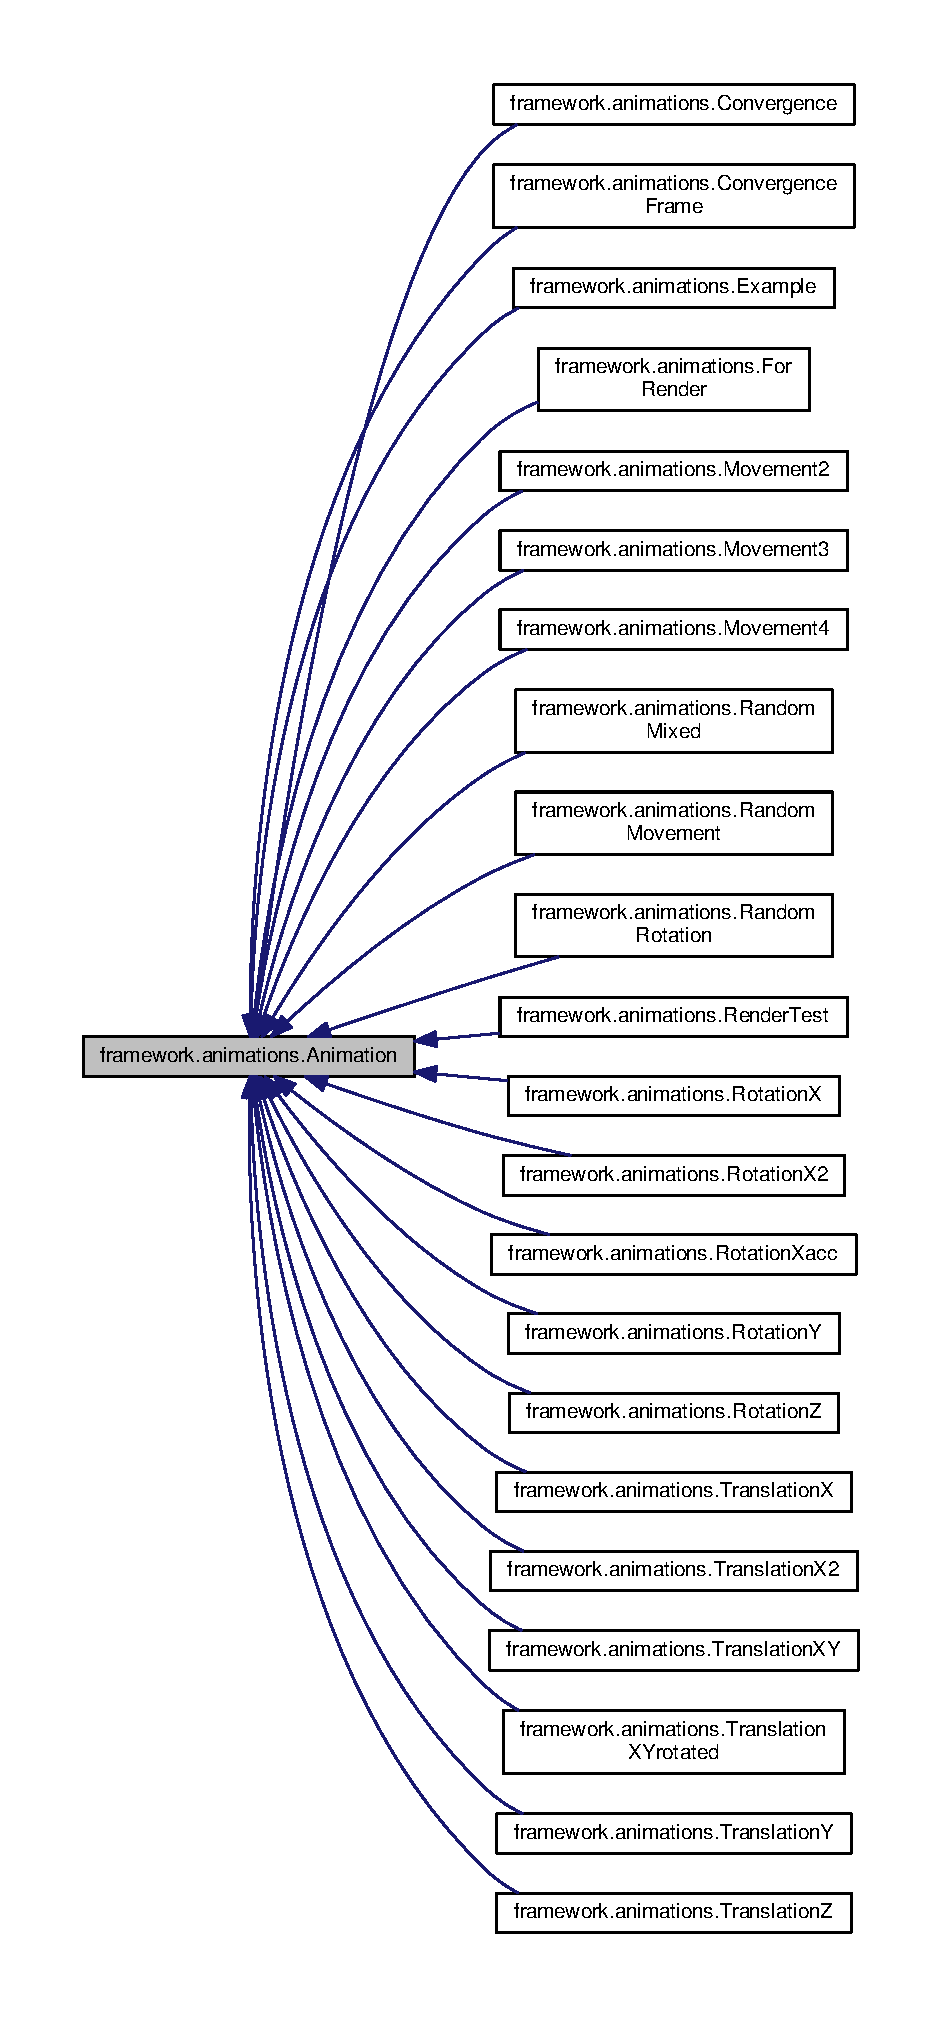
\includegraphics[height=550pt]{classframework_1_1animations_1_1Animation__inherit__graph}
\end{center}
\end{figure}
\subsection*{Public Member Functions}
\begin{DoxyCompactItemize}
\item 
def {\bfseries \+\_\+\+\_\+init\+\_\+\+\_\+} (self, bdr\+\_\+handler, blender\+\_\+object, frames)\hypertarget{classframework_1_1animations_1_1Animation_a79a2452ea3187f3364c204cded7c1d01}{}\label{classframework_1_1animations_1_1Animation_a79a2452ea3187f3364c204cded7c1d01}

\end{DoxyCompactItemize}
\subsection*{Static Public Member Functions}
\begin{DoxyCompactItemize}
\item 
def \hyperlink{classframework_1_1animations_1_1Animation_add7db1784bcb297b3572f14e2185e6cc}{get\+\_\+start\+\_\+position} ()
\item 
def \hyperlink{classframework_1_1animations_1_1Animation_a62afe4b9214c967ef11e58cf34194654}{get\+\_\+start\+\_\+rotation} ()
\end{DoxyCompactItemize}
\subsection*{Static Public Attributes}
\begin{DoxyCompactItemize}
\item 
{\bfseries obj} = None\hypertarget{classframework_1_1animations_1_1Animation_a02ddc9f994dd50dec91e9f116f4a3c56}{}\label{classframework_1_1animations_1_1Animation_a02ddc9f994dd50dec91e9f116f4a3c56}

\item 
string {\bfseries interpolation} = \char`\"{}Q\+U\+AD\char`\"{}\hypertarget{classframework_1_1animations_1_1Animation_a49075ff021d8234894db3c8830c2be6d}{}\label{classframework_1_1animations_1_1Animation_a49075ff021d8234894db3c8830c2be6d}

\end{DoxyCompactItemize}


\subsection{Member Function Documentation}
\index{framework\+::animations\+::\+Animation@{framework\+::animations\+::\+Animation}!get\+\_\+start\+\_\+position@{get\+\_\+start\+\_\+position}}
\index{get\+\_\+start\+\_\+position@{get\+\_\+start\+\_\+position}!framework\+::animations\+::\+Animation@{framework\+::animations\+::\+Animation}}
\subsubsection[{\texorpdfstring{get\+\_\+start\+\_\+position()}{get_start_position()}}]{\setlength{\rightskip}{0pt plus 5cm}def framework.\+animations.\+Animation.\+get\+\_\+start\+\_\+position (
\begin{DoxyParamCaption}
{}
\end{DoxyParamCaption}
)\hspace{0.3cm}{\ttfamily [static]}}\hypertarget{classframework_1_1animations_1_1Animation_add7db1784bcb297b3572f14e2185e6cc}{}\label{classframework_1_1animations_1_1Animation_add7db1784bcb297b3572f14e2185e6cc}
\begin{DoxyVerb}Returns the init position \end{DoxyVerb}
 \index{framework\+::animations\+::\+Animation@{framework\+::animations\+::\+Animation}!get\+\_\+start\+\_\+rotation@{get\+\_\+start\+\_\+rotation}}
\index{get\+\_\+start\+\_\+rotation@{get\+\_\+start\+\_\+rotation}!framework\+::animations\+::\+Animation@{framework\+::animations\+::\+Animation}}
\subsubsection[{\texorpdfstring{get\+\_\+start\+\_\+rotation()}{get_start_rotation()}}]{\setlength{\rightskip}{0pt plus 5cm}def framework.\+animations.\+Animation.\+get\+\_\+start\+\_\+rotation (
\begin{DoxyParamCaption}
{}
\end{DoxyParamCaption}
)\hspace{0.3cm}{\ttfamily [static]}}\hypertarget{classframework_1_1animations_1_1Animation_a62afe4b9214c967ef11e58cf34194654}{}\label{classframework_1_1animations_1_1Animation_a62afe4b9214c967ef11e58cf34194654}
\begin{DoxyVerb}Returns the init rotation \end{DoxyVerb}
 

The documentation for this class was generated from the following file\+:\begin{DoxyCompactItemize}
\item 
/home/sebastian/catkin\+\_\+ws/src/animation\+\_\+render/scripts/framework/animations.\+py\end{DoxyCompactItemize}

\hypertarget{classAnimationRender}{}\section{Animation\+Render Class Reference}
\label{classAnimationRender}\index{Animation\+Render@{Animation\+Render}}
\subsection*{Public Member Functions}
\begin{DoxyCompactItemize}
\item 
\hyperlink{classAnimationRender_add45175c946790a10451ba9cdb5caa37}{Animation\+Render} (ros\+::\+Node\+Handle $\ast$nH)
\begin{DoxyCompactList}\small\item\em \hyperlink{classAnimationRender}{Animation\+Render} Constructor. \end{DoxyCompactList}\item 
void \hyperlink{classAnimationRender_a5badc5fbb7d9c2ce6f4f9b6dda610615}{start} ()\hypertarget{classAnimationRender_a5badc5fbb7d9c2ce6f4f9b6dda610615}{}\label{classAnimationRender_a5badc5fbb7d9c2ce6f4f9b6dda610615}

\begin{DoxyCompactList}\small\item\em start Start test procedure, is called by $<$\+Start\+Test$>$ command \end{DoxyCompactList}\item 
bool \hyperlink{classAnimationRender_ae21bd75361e818fd3c10c4b9a3def277}{download\+Template\+Image} ()
\begin{DoxyCompactList}\small\item\em Download current template image. \end{DoxyCompactList}\item 
bool \hyperlink{classAnimationRender_a2b6e770e27bb976e31e19a948fcce3af}{download\+Background\+Image} ()
\begin{DoxyCompactList}\small\item\em Dwonload current background image. \end{DoxyCompactList}\end{DoxyCompactItemize}


\subsection{Constructor \& Destructor Documentation}
\index{Animation\+Render@{Animation\+Render}!Animation\+Render@{Animation\+Render}}
\index{Animation\+Render@{Animation\+Render}!Animation\+Render@{Animation\+Render}}
\subsubsection[{\texorpdfstring{Animation\+Render(ros\+::\+Node\+Handle $\ast$n\+H)}{AnimationRender(ros::NodeHandle *nH)}}]{\setlength{\rightskip}{0pt plus 5cm}Animation\+Render\+::\+Animation\+Render (
\begin{DoxyParamCaption}
\item[{ros\+::\+Node\+Handle $\ast$}]{nH}
\end{DoxyParamCaption}
)}\hypertarget{classAnimationRender_add45175c946790a10451ba9cdb5caa37}{}\label{classAnimationRender_add45175c946790a10451ba9cdb5caa37}


\hyperlink{classAnimationRender}{Animation\+Render} Constructor. 


\begin{DoxyParams}{Parameters}
{\em nH} & \\
\hline
\end{DoxyParams}


\subsection{Member Function Documentation}
\index{Animation\+Render@{Animation\+Render}!download\+Background\+Image@{download\+Background\+Image}}
\index{download\+Background\+Image@{download\+Background\+Image}!Animation\+Render@{Animation\+Render}}
\subsubsection[{\texorpdfstring{download\+Background\+Image()}{downloadBackgroundImage()}}]{\setlength{\rightskip}{0pt plus 5cm}bool Animation\+Render\+::download\+Background\+Image (
\begin{DoxyParamCaption}
{}
\end{DoxyParamCaption}
)}\hypertarget{classAnimationRender_a2b6e770e27bb976e31e19a948fcce3af}{}\label{classAnimationRender_a2b6e770e27bb976e31e19a948fcce3af}


Dwonload current background image. 

\begin{DoxyReturn}{Returns}

\end{DoxyReturn}
\index{Animation\+Render@{Animation\+Render}!download\+Template\+Image@{download\+Template\+Image}}
\index{download\+Template\+Image@{download\+Template\+Image}!Animation\+Render@{Animation\+Render}}
\subsubsection[{\texorpdfstring{download\+Template\+Image()}{downloadTemplateImage()}}]{\setlength{\rightskip}{0pt plus 5cm}bool Animation\+Render\+::download\+Template\+Image (
\begin{DoxyParamCaption}
{}
\end{DoxyParamCaption}
)}\hypertarget{classAnimationRender_ae21bd75361e818fd3c10c4b9a3def277}{}\label{classAnimationRender_ae21bd75361e818fd3c10c4b9a3def277}


Download current template image. 

\begin{DoxyReturn}{Returns}

\end{DoxyReturn}


The documentation for this class was generated from the following files\+:\begin{DoxyCompactItemize}
\item 
/home/sebastian/catkin\+\_\+ws/src/animation\+\_\+render/src/animationrender.\+h\item 
/home/sebastian/catkin\+\_\+ws/src/animation\+\_\+render/src/animationrender.\+cpp\end{DoxyCompactItemize}

\hypertarget{classframework_1_1handler_1_1BlenderHandler}{}\section{framework.\+handler.\+Blender\+Handler Class Reference}
\label{classframework_1_1handler_1_1BlenderHandler}\index{framework.\+handler.\+Blender\+Handler@{framework.\+handler.\+Blender\+Handler}}
\subsection*{Public Member Functions}
\begin{DoxyCompactItemize}
\item 
def {\bfseries \+\_\+\+\_\+init\+\_\+\+\_\+} (self, file\+\_\+path)\hypertarget{classframework_1_1handler_1_1BlenderHandler_a278091e459b1cd913866b7241edf14cd}{}\label{classframework_1_1handler_1_1BlenderHandler_a278091e459b1cd913866b7241edf14cd}

\item 
def {\bfseries create\+\_\+animation} (self, settings)\hypertarget{classframework_1_1handler_1_1BlenderHandler_a004a990458b664819ce6d8c26437a2dd}{}\label{classframework_1_1handler_1_1BlenderHandler_a004a990458b664819ce6d8c26437a2dd}

\item 
def {\bfseries set\+\_\+background\+\_\+pil} (self, image)\hypertarget{classframework_1_1handler_1_1BlenderHandler_ac27242ac703b4a73da0e10ce7c9c6a00}{}\label{classframework_1_1handler_1_1BlenderHandler_ac27242ac703b4a73da0e10ce7c9c6a00}

\item 
def {\bfseries set\+\_\+background} (self, image)\hypertarget{classframework_1_1handler_1_1BlenderHandler_a2fbbdc544511c3636244b57d3b784d39}{}\label{classframework_1_1handler_1_1BlenderHandler_a2fbbdc544511c3636244b57d3b784d39}

\item 
def {\bfseries set\+\_\+horizon\+\_\+color} (self, color)\hypertarget{classframework_1_1handler_1_1BlenderHandler_ac08044ebf42a75a6751e15b88930b4be}{}\label{classframework_1_1handler_1_1BlenderHandler_ac08044ebf42a75a6751e15b88930b4be}

\item 
def {\bfseries use\+\_\+anti\+\_\+aliasing} (self, b)\hypertarget{classframework_1_1handler_1_1BlenderHandler_a717966d6463449793037736c4a9f3d8a}{}\label{classframework_1_1handler_1_1BlenderHandler_a717966d6463449793037736c4a9f3d8a}

\item 
def {\bfseries set\+\_\+fps} (self, fps)\hypertarget{classframework_1_1handler_1_1BlenderHandler_a80a9c1be4fea298d7279b0ea0d59f2fa}{}\label{classframework_1_1handler_1_1BlenderHandler_a80a9c1be4fea298d7279b0ea0d59f2fa}

\item 
def {\bfseries set\+\_\+focal\+\_\+length} (self, focal\+\_\+length)\hypertarget{classframework_1_1handler_1_1BlenderHandler_aee68e4f46811c691c7c4389a04af7a17}{}\label{classframework_1_1handler_1_1BlenderHandler_aee68e4f46811c691c7c4389a04af7a17}

\item 
def {\bfseries set\+\_\+sensor\+\_\+width} (self, sensor\+\_\+width)\hypertarget{classframework_1_1handler_1_1BlenderHandler_a3d7e428e9c74ca2f91f6d235a9d59765}{}\label{classframework_1_1handler_1_1BlenderHandler_a3d7e428e9c74ca2f91f6d235a9d59765}

\item 
def {\bfseries set\+\_\+interpolation} (self, interpol)\hypertarget{classframework_1_1handler_1_1BlenderHandler_aa36f7737d001fce8fc70e0de3bb0eb2a}{}\label{classframework_1_1handler_1_1BlenderHandler_aa36f7737d001fce8fc70e0de3bb0eb2a}

\item 
def {\bfseries use\+\_\+environment\+\_\+light} (self, b)\hypertarget{classframework_1_1handler_1_1BlenderHandler_a419f9b3bedad6ac24629c69f7436209a}{}\label{classframework_1_1handler_1_1BlenderHandler_a419f9b3bedad6ac24629c69f7436209a}

\item 
def {\bfseries set\+\_\+environment\+\_\+energy} (self, e)\hypertarget{classframework_1_1handler_1_1BlenderHandler_ab7c96e5ed9b2097bb1156bbd687c64b7}{}\label{classframework_1_1handler_1_1BlenderHandler_ab7c96e5ed9b2097bb1156bbd687c64b7}

\item 
def {\bfseries render\+\_\+and\+\_\+save} (self, path=None)\hypertarget{classframework_1_1handler_1_1BlenderHandler_a59256cba8493354e093157dee32a54eb}{}\label{classframework_1_1handler_1_1BlenderHandler_a59256cba8493354e093157dee32a54eb}

\item 
def {\bfseries animation\+\_\+and\+\_\+save} (self, path=None)\hypertarget{classframework_1_1handler_1_1BlenderHandler_a9f6cb77a04f2498cbc73753cc6d7e1b8}{}\label{classframework_1_1handler_1_1BlenderHandler_a9f6cb77a04f2498cbc73753cc6d7e1b8}

\end{DoxyCompactItemize}
\subsection*{Static Public Member Functions}
\begin{DoxyCompactItemize}
\item 
def {\bfseries set\+\_\+resolution} (x, y)\hypertarget{classframework_1_1handler_1_1BlenderHandler_abfb34ad8570c3b190aa7d0010174e17f}{}\label{classframework_1_1handler_1_1BlenderHandler_abfb34ad8570c3b190aa7d0010174e17f}

\end{DoxyCompactItemize}
\subsection*{Static Public Attributes}
\begin{DoxyCompactItemize}
\item 
{\bfseries file\+\_\+path} = None\hypertarget{classframework_1_1handler_1_1BlenderHandler_ac64148d881bc152a0e378e25529db11c}{}\label{classframework_1_1handler_1_1BlenderHandler_ac64148d881bc152a0e378e25529db11c}

\item 
{\bfseries world} = None\hypertarget{classframework_1_1handler_1_1BlenderHandler_a416cfd48d0e660438a8c3c258cebb5b8}{}\label{classframework_1_1handler_1_1BlenderHandler_a416cfd48d0e660438a8c3c258cebb5b8}

\item 
{\bfseries scene} = None\hypertarget{classframework_1_1handler_1_1BlenderHandler_a300781bdf7564687a54e0c0a441e72d8}{}\label{classframework_1_1handler_1_1BlenderHandler_a300781bdf7564687a54e0c0a441e72d8}

\item 
{\bfseries camera} = None\hypertarget{classframework_1_1handler_1_1BlenderHandler_a42cc53178c79726a87a2107d7318f8f0}{}\label{classframework_1_1handler_1_1BlenderHandler_a42cc53178c79726a87a2107d7318f8f0}

\item 
{\bfseries bgr\+\_\+img} = None\hypertarget{classframework_1_1handler_1_1BlenderHandler_a887c45867c4ad1dd00a0b1a3ad996d05}{}\label{classframework_1_1handler_1_1BlenderHandler_a887c45867c4ad1dd00a0b1a3ad996d05}

\item 
{\bfseries bgr\+\_\+tex} = None\hypertarget{classframework_1_1handler_1_1BlenderHandler_a23b723c2fa0081e00ef802a7af201861}{}\label{classframework_1_1handler_1_1BlenderHandler_a23b723c2fa0081e00ef802a7af201861}

\item 
{\bfseries bgr\+\_\+tex\+\_\+slot} = None\hypertarget{classframework_1_1handler_1_1BlenderHandler_a39c8cdffeeb9d4f5f07b502ddaa3d2d0}{}\label{classframework_1_1handler_1_1BlenderHandler_a39c8cdffeeb9d4f5f07b502ddaa3d2d0}

\end{DoxyCompactItemize}


The documentation for this class was generated from the following file\+:\begin{DoxyCompactItemize}
\item 
/home/sebastian/catkin\+\_\+ws/src/animation\+\_\+render/scripts/framework/handler.\+py\end{DoxyCompactItemize}

\hypertarget{classframework_1_1objects_1_1BlenderObject}{}\section{framework.\+objects.\+Blender\+Object Class Reference}
\label{classframework_1_1objects_1_1BlenderObject}\index{framework.\+objects.\+Blender\+Object@{framework.\+objects.\+Blender\+Object}}


Inheritance diagram for framework.\+objects.\+Blender\+Object\+:
\nopagebreak
\begin{figure}[H]
\begin{center}
\leavevmode
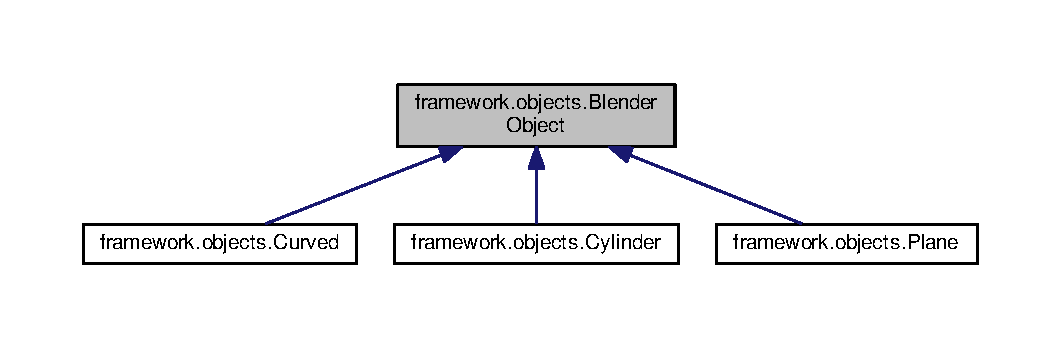
\includegraphics[width=350pt]{classframework_1_1objects_1_1BlenderObject__inherit__graph}
\end{center}
\end{figure}
\subsection*{Public Member Functions}
\begin{DoxyCompactItemize}
\item 
def {\bfseries \+\_\+\+\_\+init\+\_\+\+\_\+} (self, name, image=None)\hypertarget{classframework_1_1objects_1_1BlenderObject_a88d49788968741d6d37f20f38900b451}{}\label{classframework_1_1objects_1_1BlenderObject_a88d49788968741d6d37f20f38900b451}

\item 
def {\bfseries set\+\_\+location} (self, loc)\hypertarget{classframework_1_1objects_1_1BlenderObject_a3ea36025c4d18f76a18f937aacb38a66}{}\label{classframework_1_1objects_1_1BlenderObject_a3ea36025c4d18f76a18f937aacb38a66}

\item 
def {\bfseries set\+\_\+rotation} (self, rot)\hypertarget{classframework_1_1objects_1_1BlenderObject_ada16595efb0f086a7924b3f66de4c89b}{}\label{classframework_1_1objects_1_1BlenderObject_ada16595efb0f086a7924b3f66de4c89b}

\item 
def {\bfseries set\+\_\+image} (self, image)\hypertarget{classframework_1_1objects_1_1BlenderObject_aad4e39d8a1d94e9ce07884aa1db1c336}{}\label{classframework_1_1objects_1_1BlenderObject_aad4e39d8a1d94e9ce07884aa1db1c336}

\item 
def {\bfseries keyframe\+\_\+insert} (self, keyframe\+\_\+type, frame)\hypertarget{classframework_1_1objects_1_1BlenderObject_ac14208aa974016c67fdfa52bf296859e}{}\label{classframework_1_1objects_1_1BlenderObject_ac14208aa974016c67fdfa52bf296859e}

\end{DoxyCompactItemize}
\subsection*{Static Public Attributes}
\begin{DoxyCompactItemize}
\item 
{\bfseries name} = None\hypertarget{classframework_1_1objects_1_1BlenderObject_aa3cf78717bf12612ae9019de061be874}{}\label{classframework_1_1objects_1_1BlenderObject_aa3cf78717bf12612ae9019de061be874}

\item 
{\bfseries obj} = None\hypertarget{classframework_1_1objects_1_1BlenderObject_ac6552fd16b067cd39a3bf80f9b20f775}{}\label{classframework_1_1objects_1_1BlenderObject_ac6552fd16b067cd39a3bf80f9b20f775}

\item 
{\bfseries img} = None\hypertarget{classframework_1_1objects_1_1BlenderObject_a735951a1c2c48406db49a8597fb43f52}{}\label{classframework_1_1objects_1_1BlenderObject_a735951a1c2c48406db49a8597fb43f52}

\item 
{\bfseries tex} = None\hypertarget{classframework_1_1objects_1_1BlenderObject_aba326a9581bf8d012dfff6d8b7851cf6}{}\label{classframework_1_1objects_1_1BlenderObject_aba326a9581bf8d012dfff6d8b7851cf6}

\item 
{\bfseries mat} = None\hypertarget{classframework_1_1objects_1_1BlenderObject_a3af924160e7ac996b2e22cad7aabb340}{}\label{classframework_1_1objects_1_1BlenderObject_a3af924160e7ac996b2e22cad7aabb340}

\end{DoxyCompactItemize}


The documentation for this class was generated from the following file\+:\begin{DoxyCompactItemize}
\item 
/home/sebastian/catkin\+\_\+ws/src/animation\+\_\+render/scripts/framework/objects.\+py\end{DoxyCompactItemize}

\hypertarget{classframework_1_1animations_1_1Convergence}{}\section{framework.\+animations.\+Convergence Class Reference}
\label{classframework_1_1animations_1_1Convergence}\index{framework.\+animations.\+Convergence@{framework.\+animations.\+Convergence}}


Inheritance diagram for framework.\+animations.\+Convergence\+:
\nopagebreak
\begin{figure}[H]
\begin{center}
\leavevmode
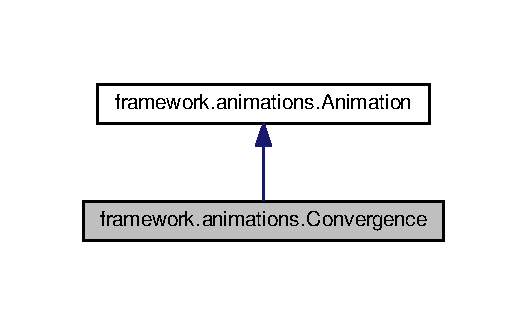
\includegraphics[width=253pt]{classframework_1_1animations_1_1Convergence__inherit__graph}
\end{center}
\end{figure}


Collaboration diagram for framework.\+animations.\+Convergence\+:
\nopagebreak
\begin{figure}[H]
\begin{center}
\leavevmode
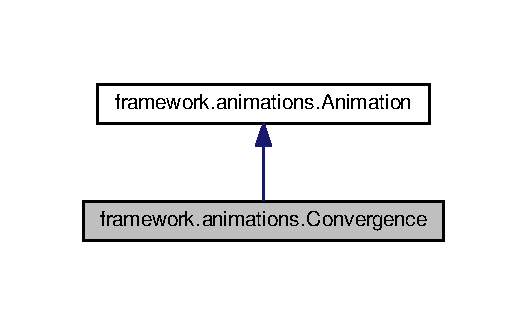
\includegraphics[width=253pt]{classframework_1_1animations_1_1Convergence__coll__graph}
\end{center}
\end{figure}
\subsection*{Public Member Functions}
\begin{DoxyCompactItemize}
\item 
def {\bfseries \+\_\+\+\_\+init\+\_\+\+\_\+} (self, bdr\+\_\+handler, blender\+\_\+object, frames)\hypertarget{classframework_1_1animations_1_1Convergence_abe3ee04c7e1218fdad4dc14961c5504f}{}\label{classframework_1_1animations_1_1Convergence_abe3ee04c7e1218fdad4dc14961c5504f}

\end{DoxyCompactItemize}
\subsection*{Static Public Member Functions}
\begin{DoxyCompactItemize}
\item 
def {\bfseries get\+\_\+start\+\_\+position} ()\hypertarget{classframework_1_1animations_1_1Convergence_a444d7b2174ec2a3d2f67e9d0614fa688}{}\label{classframework_1_1animations_1_1Convergence_a444d7b2174ec2a3d2f67e9d0614fa688}

\item 
def {\bfseries get\+\_\+start\+\_\+rotation} ()\hypertarget{classframework_1_1animations_1_1Convergence_aeac8590cb8af3818d0e30719bf6a7da8}{}\label{classframework_1_1animations_1_1Convergence_aeac8590cb8af3818d0e30719bf6a7da8}

\end{DoxyCompactItemize}
\subsection*{Additional Inherited Members}


The documentation for this class was generated from the following file\+:\begin{DoxyCompactItemize}
\item 
/home/sebastian/catkin\+\_\+ws/src/animation\+\_\+render/scripts/framework/animations.\+py\end{DoxyCompactItemize}

\hypertarget{classframework_1_1animations_1_1ConvergenceFrame}{}\section{framework.\+animations.\+Convergence\+Frame Class Reference}
\label{classframework_1_1animations_1_1ConvergenceFrame}\index{framework.\+animations.\+Convergence\+Frame@{framework.\+animations.\+Convergence\+Frame}}


Inheritance diagram for framework.\+animations.\+Convergence\+Frame\+:
\nopagebreak
\begin{figure}[H]
\begin{center}
\leavevmode
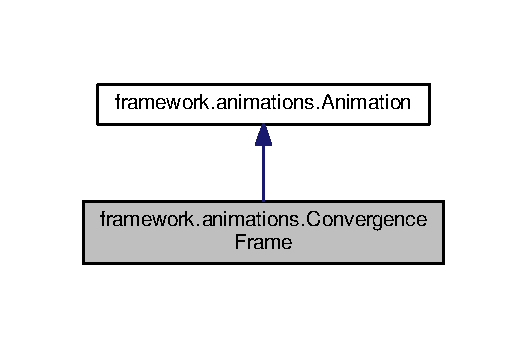
\includegraphics[width=253pt]{classframework_1_1animations_1_1ConvergenceFrame__inherit__graph}
\end{center}
\end{figure}


Collaboration diagram for framework.\+animations.\+Convergence\+Frame\+:
\nopagebreak
\begin{figure}[H]
\begin{center}
\leavevmode
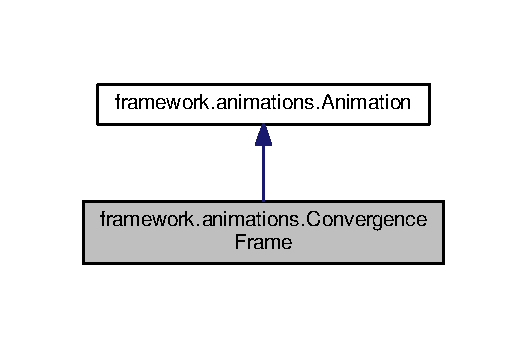
\includegraphics[width=253pt]{classframework_1_1animations_1_1ConvergenceFrame__coll__graph}
\end{center}
\end{figure}
\subsection*{Public Member Functions}
\begin{DoxyCompactItemize}
\item 
def {\bfseries \+\_\+\+\_\+init\+\_\+\+\_\+} (self, bdr\+\_\+handler, blender\+\_\+object, frames)\hypertarget{classframework_1_1animations_1_1ConvergenceFrame_a66e82c5c5b56b3efd47b05b93ad5caec}{}\label{classframework_1_1animations_1_1ConvergenceFrame_a66e82c5c5b56b3efd47b05b93ad5caec}

\end{DoxyCompactItemize}
\subsection*{Static Public Member Functions}
\begin{DoxyCompactItemize}
\item 
def {\bfseries get\+\_\+start\+\_\+position} ()\hypertarget{classframework_1_1animations_1_1ConvergenceFrame_ab33604a6f370aceadb142caebb2e85a4}{}\label{classframework_1_1animations_1_1ConvergenceFrame_ab33604a6f370aceadb142caebb2e85a4}

\item 
def {\bfseries get\+\_\+start\+\_\+rotation} ()\hypertarget{classframework_1_1animations_1_1ConvergenceFrame_a7db583b84ccb0203f1815ca259781762}{}\label{classframework_1_1animations_1_1ConvergenceFrame_a7db583b84ccb0203f1815ca259781762}

\end{DoxyCompactItemize}
\subsection*{Additional Inherited Members}


The documentation for this class was generated from the following file\+:\begin{DoxyCompactItemize}
\item 
/home/sebastian/catkin\+\_\+ws/src/animation\+\_\+render/scripts/framework/animations.\+py\end{DoxyCompactItemize}

\hypertarget{classframework_1_1objects_1_1Curved}{}\section{framework.\+objects.\+Curved Class Reference}
\label{classframework_1_1objects_1_1Curved}\index{framework.\+objects.\+Curved@{framework.\+objects.\+Curved}}


Inheritance diagram for framework.\+objects.\+Curved\+:
\nopagebreak
\begin{figure}[H]
\begin{center}
\leavevmode
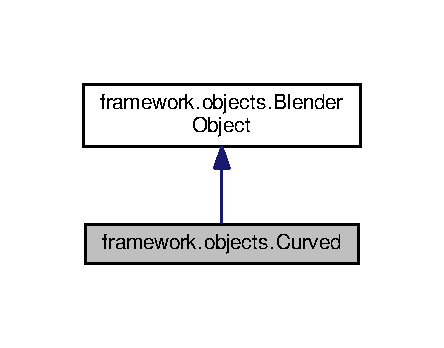
\includegraphics[width=213pt]{classframework_1_1objects_1_1Curved__inherit__graph}
\end{center}
\end{figure}


Collaboration diagram for framework.\+objects.\+Curved\+:
\nopagebreak
\begin{figure}[H]
\begin{center}
\leavevmode
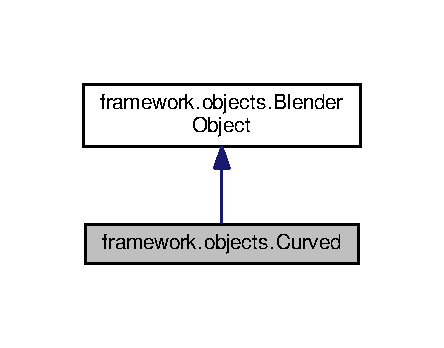
\includegraphics[width=213pt]{classframework_1_1objects_1_1Curved__coll__graph}
\end{center}
\end{figure}
\subsection*{Public Member Functions}
\begin{DoxyCompactItemize}
\item 
def {\bfseries \+\_\+\+\_\+init\+\_\+\+\_\+} (self, p1, p2, p3, image=None)\hypertarget{classframework_1_1objects_1_1Curved_acf37a88ee28b6727721ee4cf0e8bac05}{}\label{classframework_1_1objects_1_1Curved_acf37a88ee28b6727721ee4cf0e8bac05}

\end{DoxyCompactItemize}
\subsection*{Public Attributes}
\begin{DoxyCompactItemize}
\item 
{\bfseries length}\hypertarget{classframework_1_1objects_1_1Curved_ae0c75c8d075c4e5fd6cfcaebb94a9239}{}\label{classframework_1_1objects_1_1Curved_ae0c75c8d075c4e5fd6cfcaebb94a9239}

\item 
{\bfseries radius}\hypertarget{classframework_1_1objects_1_1Curved_af386b37a16e13812074cdf182f44f35a}{}\label{classframework_1_1objects_1_1Curved_af386b37a16e13812074cdf182f44f35a}

\item 
{\bfseries n\+Faces}\hypertarget{classframework_1_1objects_1_1Curved_a3e82a8661ab49e6773ff76f4f5f58838}{}\label{classframework_1_1objects_1_1Curved_a3e82a8661ab49e6773ff76f4f5f58838}

\end{DoxyCompactItemize}
\subsection*{Static Public Attributes}
\begin{DoxyCompactItemize}
\item 
int {\bfseries n\+Faces} = 100\hypertarget{classframework_1_1objects_1_1Curved_a3972fd941e1871a932e2e0385d6a7dcd}{}\label{classframework_1_1objects_1_1Curved_a3972fd941e1871a932e2e0385d6a7dcd}

\item 
int {\bfseries radius} = 1\hypertarget{classframework_1_1objects_1_1Curved_a90d781959c8b1b178dc630a93a447b10}{}\label{classframework_1_1objects_1_1Curved_a90d781959c8b1b178dc630a93a447b10}

\item 
int {\bfseries length} = 5\hypertarget{classframework_1_1objects_1_1Curved_acd85658172267dfaecf19a0065b54b35}{}\label{classframework_1_1objects_1_1Curved_acd85658172267dfaecf19a0065b54b35}

\item 
list {\bfseries top\+\_\+face} = \mbox{[}$\,$\mbox{]}\hypertarget{classframework_1_1objects_1_1Curved_a946c0d36574f56c770b55bd56097bfe1}{}\label{classframework_1_1objects_1_1Curved_a946c0d36574f56c770b55bd56097bfe1}

\item 
list {\bfseries bot\+\_\+face} = \mbox{[}$\,$\mbox{]}\hypertarget{classframework_1_1objects_1_1Curved_aca487246845b97d0b0ed43d3ef4574cc}{}\label{classframework_1_1objects_1_1Curved_aca487246845b97d0b0ed43d3ef4574cc}

\item 
{\bfseries mesh} = None\hypertarget{classframework_1_1objects_1_1Curved_a6ca07eac8d916d95552fa65cf8d106e4}{}\label{classframework_1_1objects_1_1Curved_a6ca07eac8d916d95552fa65cf8d106e4}

\end{DoxyCompactItemize}


The documentation for this class was generated from the following file\+:\begin{DoxyCompactItemize}
\item 
/home/sebastian/catkin\+\_\+ws/src/animation\+\_\+render/scripts/framework/objects.\+py\end{DoxyCompactItemize}

\hypertarget{classframework_1_1objects_1_1Cylinder}{}\section{framework.\+objects.\+Cylinder Class Reference}
\label{classframework_1_1objects_1_1Cylinder}\index{framework.\+objects.\+Cylinder@{framework.\+objects.\+Cylinder}}


Inheritance diagram for framework.\+objects.\+Cylinder\+:
\nopagebreak
\begin{figure}[H]
\begin{center}
\leavevmode
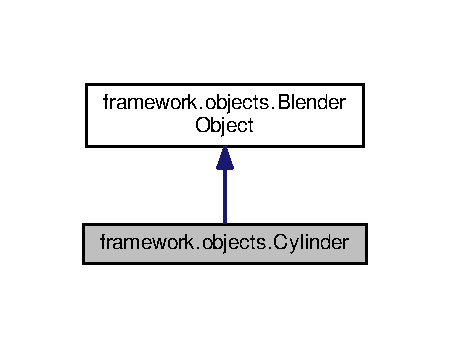
\includegraphics[width=216pt]{classframework_1_1objects_1_1Cylinder__inherit__graph}
\end{center}
\end{figure}


Collaboration diagram for framework.\+objects.\+Cylinder\+:
\nopagebreak
\begin{figure}[H]
\begin{center}
\leavevmode
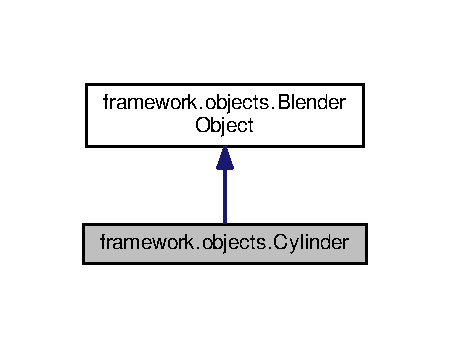
\includegraphics[width=216pt]{classframework_1_1objects_1_1Cylinder__coll__graph}
\end{center}
\end{figure}
\subsection*{Public Member Functions}
\begin{DoxyCompactItemize}
\item 
def {\bfseries \+\_\+\+\_\+init\+\_\+\+\_\+} (self, p1, p2, p3, image=None)\hypertarget{classframework_1_1objects_1_1Cylinder_a78c169cac92f2143b6ee017361061656}{}\label{classframework_1_1objects_1_1Cylinder_a78c169cac92f2143b6ee017361061656}

\end{DoxyCompactItemize}
\subsection*{Public Attributes}
\begin{DoxyCompactItemize}
\item 
{\bfseries length}\hypertarget{classframework_1_1objects_1_1Cylinder_ade1ff97da5bc19544d565274430cab5b}{}\label{classframework_1_1objects_1_1Cylinder_ade1ff97da5bc19544d565274430cab5b}

\item 
{\bfseries radius}\hypertarget{classframework_1_1objects_1_1Cylinder_a53c5ca9d37cc5afd5435cf1c1d798351}{}\label{classframework_1_1objects_1_1Cylinder_a53c5ca9d37cc5afd5435cf1c1d798351}

\item 
{\bfseries n\+Faces}\hypertarget{classframework_1_1objects_1_1Cylinder_aa17ab2f31ca74b4ab48ee401659aa44f}{}\label{classframework_1_1objects_1_1Cylinder_aa17ab2f31ca74b4ab48ee401659aa44f}

\end{DoxyCompactItemize}
\subsection*{Static Public Attributes}
\begin{DoxyCompactItemize}
\item 
int {\bfseries n\+Faces} = 100\hypertarget{classframework_1_1objects_1_1Cylinder_a636ea80f7e9523f5fdb17730fa704c6c}{}\label{classframework_1_1objects_1_1Cylinder_a636ea80f7e9523f5fdb17730fa704c6c}

\item 
int {\bfseries radius} = 1\hypertarget{classframework_1_1objects_1_1Cylinder_ab7657331b2cdd7d3457089c789829f96}{}\label{classframework_1_1objects_1_1Cylinder_ab7657331b2cdd7d3457089c789829f96}

\item 
int {\bfseries length} = 5\hypertarget{classframework_1_1objects_1_1Cylinder_a2f920bc718c300a1d72b41084bfc4cce}{}\label{classframework_1_1objects_1_1Cylinder_a2f920bc718c300a1d72b41084bfc4cce}

\item 
list {\bfseries top\+\_\+face} = \mbox{[}$\,$\mbox{]}\hypertarget{classframework_1_1objects_1_1Cylinder_aaee8cc61b5dd561a6cfd2b25a14f8255}{}\label{classframework_1_1objects_1_1Cylinder_aaee8cc61b5dd561a6cfd2b25a14f8255}

\item 
list {\bfseries bot\+\_\+face} = \mbox{[}$\,$\mbox{]}\hypertarget{classframework_1_1objects_1_1Cylinder_a90785a332a3fa55735976464dbd34b16}{}\label{classframework_1_1objects_1_1Cylinder_a90785a332a3fa55735976464dbd34b16}

\item 
{\bfseries mesh} = None\hypertarget{classframework_1_1objects_1_1Cylinder_a00823e3e693f6684c3fe3607990eea02}{}\label{classframework_1_1objects_1_1Cylinder_a00823e3e693f6684c3fe3607990eea02}

\end{DoxyCompactItemize}


The documentation for this class was generated from the following file\+:\begin{DoxyCompactItemize}
\item 
/home/sebastian/catkin\+\_\+ws/src/animation\+\_\+render/scripts/framework/objects.\+py\end{DoxyCompactItemize}

\hypertarget{classframework_1_1animations_1_1Example}{}\section{framework.\+animations.\+Example Class Reference}
\label{classframework_1_1animations_1_1Example}\index{framework.\+animations.\+Example@{framework.\+animations.\+Example}}


Inheritance diagram for framework.\+animations.\+Example\+:
\nopagebreak
\begin{figure}[H]
\begin{center}
\leavevmode
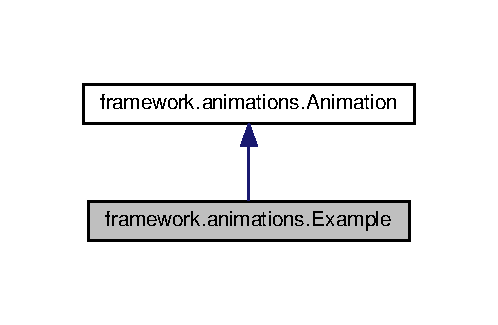
\includegraphics[width=239pt]{classframework_1_1animations_1_1Example__inherit__graph}
\end{center}
\end{figure}


Collaboration diagram for framework.\+animations.\+Example\+:
\nopagebreak
\begin{figure}[H]
\begin{center}
\leavevmode
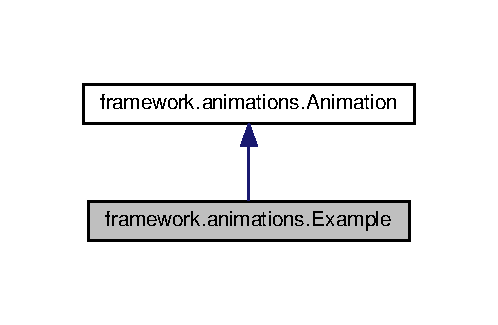
\includegraphics[width=239pt]{classframework_1_1animations_1_1Example__coll__graph}
\end{center}
\end{figure}
\subsection*{Public Member Functions}
\begin{DoxyCompactItemize}
\item 
def {\bfseries \+\_\+\+\_\+init\+\_\+\+\_\+} (self, bdr\+\_\+handler, blender\+\_\+object, frames)\hypertarget{classframework_1_1animations_1_1Example_a065bdcf4353bb897272e0105bc31737e}{}\label{classframework_1_1animations_1_1Example_a065bdcf4353bb897272e0105bc31737e}

\end{DoxyCompactItemize}
\subsection*{Static Public Member Functions}
\begin{DoxyCompactItemize}
\item 
def {\bfseries get\+\_\+start\+\_\+position} ()\hypertarget{classframework_1_1animations_1_1Example_aa213ab340b6a42b5541758c569bdad5d}{}\label{classframework_1_1animations_1_1Example_aa213ab340b6a42b5541758c569bdad5d}

\item 
def {\bfseries get\+\_\+start\+\_\+rotation} ()\hypertarget{classframework_1_1animations_1_1Example_a62a42f30cd28f5ea74c22be79473eacc}{}\label{classframework_1_1animations_1_1Example_a62a42f30cd28f5ea74c22be79473eacc}

\end{DoxyCompactItemize}
\subsection*{Static Public Attributes}
\begin{DoxyCompactItemize}
\item 
string {\bfseries interpolation} = \textquotesingle{}L\+I\+N\+E\+AR\textquotesingle{}\hypertarget{classframework_1_1animations_1_1Example_aadde8ecc16566cf29faa2245ff07d245}{}\label{classframework_1_1animations_1_1Example_aadde8ecc16566cf29faa2245ff07d245}

\end{DoxyCompactItemize}


The documentation for this class was generated from the following file\+:\begin{DoxyCompactItemize}
\item 
/home/sebastian/catkin\+\_\+ws/src/animation\+\_\+render/scripts/framework/animations.\+py\end{DoxyCompactItemize}

\hypertarget{classframework_1_1animations_1_1ForRender}{}\section{framework.\+animations.\+For\+Render Class Reference}
\label{classframework_1_1animations_1_1ForRender}\index{framework.\+animations.\+For\+Render@{framework.\+animations.\+For\+Render}}


Inheritance diagram for framework.\+animations.\+For\+Render\+:
\nopagebreak
\begin{figure}[H]
\begin{center}
\leavevmode
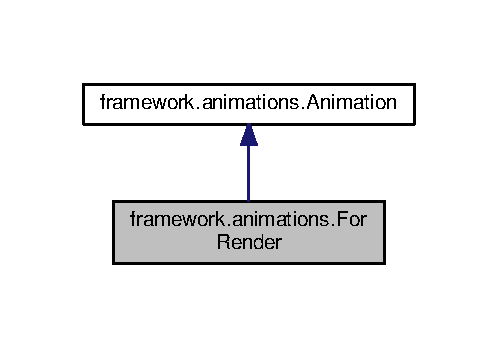
\includegraphics[width=239pt]{classframework_1_1animations_1_1ForRender__inherit__graph}
\end{center}
\end{figure}


Collaboration diagram for framework.\+animations.\+For\+Render\+:
\nopagebreak
\begin{figure}[H]
\begin{center}
\leavevmode
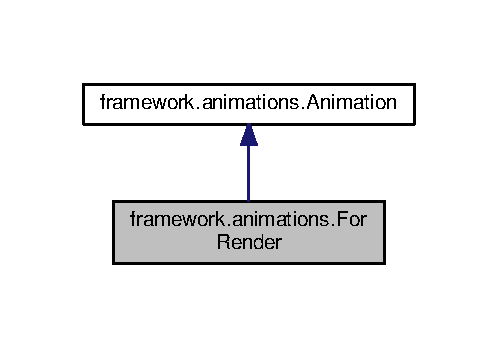
\includegraphics[width=239pt]{classframework_1_1animations_1_1ForRender__coll__graph}
\end{center}
\end{figure}
\subsection*{Public Member Functions}
\begin{DoxyCompactItemize}
\item 
def {\bfseries \+\_\+\+\_\+init\+\_\+\+\_\+} (self, bdr\+\_\+handler, blender\+\_\+object, frames)\hypertarget{classframework_1_1animations_1_1ForRender_a4a4b41229fad58fe5d672451b37f3798}{}\label{classframework_1_1animations_1_1ForRender_a4a4b41229fad58fe5d672451b37f3798}

\end{DoxyCompactItemize}
\subsection*{Static Public Member Functions}
\begin{DoxyCompactItemize}
\item 
def {\bfseries get\+\_\+start\+\_\+position} ()\hypertarget{classframework_1_1animations_1_1ForRender_a599aadfcdf3ca0d3bdd08217a1d0a648}{}\label{classframework_1_1animations_1_1ForRender_a599aadfcdf3ca0d3bdd08217a1d0a648}

\item 
def {\bfseries get\+\_\+start\+\_\+rotation} ()\hypertarget{classframework_1_1animations_1_1ForRender_affe4cb9f8f25a3710e8fab94615a2dd0}{}\label{classframework_1_1animations_1_1ForRender_affe4cb9f8f25a3710e8fab94615a2dd0}

\end{DoxyCompactItemize}
\subsection*{Additional Inherited Members}


The documentation for this class was generated from the following file\+:\begin{DoxyCompactItemize}
\item 
/home/sebastian/catkin\+\_\+ws/src/animation\+\_\+render/scripts/framework/animations.\+py\end{DoxyCompactItemize}

\hypertarget{classframework_1_1handler_1_1ImageHandler}{}\section{framework.\+handler.\+Image\+Handler Class Reference}
\label{classframework_1_1handler_1_1ImageHandler}\index{framework.\+handler.\+Image\+Handler@{framework.\+handler.\+Image\+Handler}}
\subsection*{Public Member Functions}
\begin{DoxyCompactItemize}
\item 
def {\bfseries \+\_\+\+\_\+init\+\_\+\+\_\+} (self, api\+\_\+key, api\+\_\+secret, n\+\_\+images)\hypertarget{classframework_1_1handler_1_1ImageHandler_a8afd09c10e7e3aef500c0fbe88b14459}{}\label{classframework_1_1handler_1_1ImageHandler_a8afd09c10e7e3aef500c0fbe88b14459}

\item 
def {\bfseries load\+\_\+photos\+\_\+same\+\_\+keywords} (self, keywords)\hypertarget{classframework_1_1handler_1_1ImageHandler_a7b7f852de1f4780cd6b39b69b0158d0e}{}\label{classframework_1_1handler_1_1ImageHandler_a7b7f852de1f4780cd6b39b69b0158d0e}

\item 
def {\bfseries load\+\_\+photos\+\_\+different\+\_\+keywords} (self, bgr\+\_\+keywords, tpl\+\_\+keywords)\hypertarget{classframework_1_1handler_1_1ImageHandler_a213a5aead7a1e2d1516d63f4f9b910c3}{}\label{classframework_1_1handler_1_1ImageHandler_a213a5aead7a1e2d1516d63f4f9b910c3}

\item 
def {\bfseries get\+\_\+background} (self)\hypertarget{classframework_1_1handler_1_1ImageHandler_aa65a782baf396143d02b6276665b0d96}{}\label{classframework_1_1handler_1_1ImageHandler_aa65a782baf396143d02b6276665b0d96}

\item 
def {\bfseries get\+\_\+template} (self)\hypertarget{classframework_1_1handler_1_1ImageHandler_aec6aa31081de5c55c960dcbef8befaf6}{}\label{classframework_1_1handler_1_1ImageHandler_aec6aa31081de5c55c960dcbef8befaf6}

\end{DoxyCompactItemize}
\subsection*{Public Attributes}
\begin{DoxyCompactItemize}
\item 
{\bfseries n\+\_\+images}\hypertarget{classframework_1_1handler_1_1ImageHandler_aa873eb32032c51d4f9dd4eb42bd24410}{}\label{classframework_1_1handler_1_1ImageHandler_aa873eb32032c51d4f9dd4eb42bd24410}

\end{DoxyCompactItemize}
\subsection*{Static Public Attributes}
\begin{DoxyCompactItemize}
\item 
{\bfseries api} = None\hypertarget{classframework_1_1handler_1_1ImageHandler_a86dde1ca5b4ecfe2968ac3f246097fea}{}\label{classframework_1_1handler_1_1ImageHandler_a86dde1ca5b4ecfe2968ac3f246097fea}

\item 
{\bfseries api\+\_\+key} = None\hypertarget{classframework_1_1handler_1_1ImageHandler_a362797523d6c9a2a29afa3c15347c3ae}{}\label{classframework_1_1handler_1_1ImageHandler_a362797523d6c9a2a29afa3c15347c3ae}

\item 
{\bfseries api\+\_\+secret} = None\hypertarget{classframework_1_1handler_1_1ImageHandler_a5766f50fd18d6d26cabc633ff9265288}{}\label{classframework_1_1handler_1_1ImageHandler_a5766f50fd18d6d26cabc633ff9265288}

\item 
{\bfseries tpl\+\_\+photos} = list()\hypertarget{classframework_1_1handler_1_1ImageHandler_a86f400d5dc00384ea4e689c9f0f2a337}{}\label{classframework_1_1handler_1_1ImageHandler_a86f400d5dc00384ea4e689c9f0f2a337}

\item 
{\bfseries bgr\+\_\+photos} = list()\hypertarget{classframework_1_1handler_1_1ImageHandler_a77d7b13fafe47b8ef63aca1d981557b6}{}\label{classframework_1_1handler_1_1ImageHandler_a77d7b13fafe47b8ef63aca1d981557b6}

\item 
int {\bfseries n\+\_\+images} = 100\hypertarget{classframework_1_1handler_1_1ImageHandler_ab73d3eb32f34dec641f79b420db358f4}{}\label{classframework_1_1handler_1_1ImageHandler_ab73d3eb32f34dec641f79b420db358f4}

\end{DoxyCompactItemize}


The documentation for this class was generated from the following file\+:\begin{DoxyCompactItemize}
\item 
/home/sebastian/catkin\+\_\+ws/src/animation\+\_\+render/scripts/framework/handler.\+py\end{DoxyCompactItemize}

\hypertarget{classframework_1_1animations_1_1Movement2}{}\section{framework.\+animations.\+Movement2 Class Reference}
\label{classframework_1_1animations_1_1Movement2}\index{framework.\+animations.\+Movement2@{framework.\+animations.\+Movement2}}


Inheritance diagram for framework.\+animations.\+Movement2\+:
\nopagebreak
\begin{figure}[H]
\begin{center}
\leavevmode
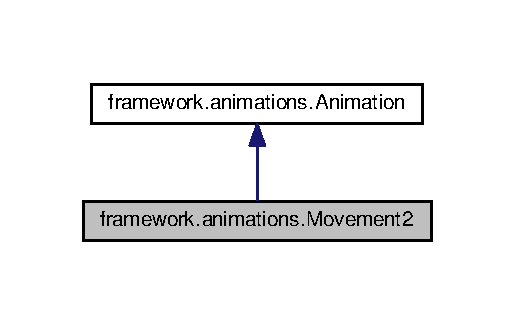
\includegraphics[width=247pt]{classframework_1_1animations_1_1Movement2__inherit__graph}
\end{center}
\end{figure}


Collaboration diagram for framework.\+animations.\+Movement2\+:
\nopagebreak
\begin{figure}[H]
\begin{center}
\leavevmode
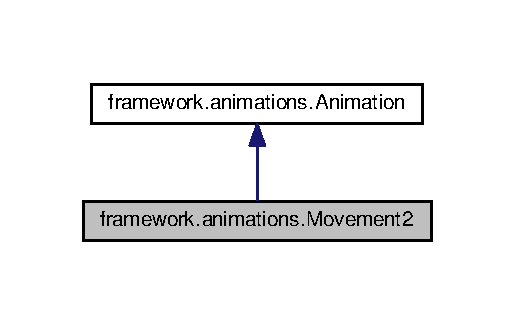
\includegraphics[width=247pt]{classframework_1_1animations_1_1Movement2__coll__graph}
\end{center}
\end{figure}
\subsection*{Public Member Functions}
\begin{DoxyCompactItemize}
\item 
def {\bfseries \+\_\+\+\_\+init\+\_\+\+\_\+} (self, bdr\+\_\+handler, blender\+\_\+object, frames)\hypertarget{classframework_1_1animations_1_1Movement2_aecd510c25bd0ee4ccb398b9fbe85826f}{}\label{classframework_1_1animations_1_1Movement2_aecd510c25bd0ee4ccb398b9fbe85826f}

\end{DoxyCompactItemize}
\subsection*{Static Public Member Functions}
\begin{DoxyCompactItemize}
\item 
def {\bfseries get\+\_\+start\+\_\+position} ()\hypertarget{classframework_1_1animations_1_1Movement2_affe82db517fb606152cd126ecc1b4c23}{}\label{classframework_1_1animations_1_1Movement2_affe82db517fb606152cd126ecc1b4c23}

\item 
def {\bfseries get\+\_\+start\+\_\+rotation} ()\hypertarget{classframework_1_1animations_1_1Movement2_a7ada53f15d4cd0139e809dce4da8b4f1}{}\label{classframework_1_1animations_1_1Movement2_a7ada53f15d4cd0139e809dce4da8b4f1}

\end{DoxyCompactItemize}
\subsection*{Static Public Attributes}
\begin{DoxyCompactItemize}
\item 
string {\bfseries interpolation} = \textquotesingle{}L\+I\+N\+E\+AR\textquotesingle{}\hypertarget{classframework_1_1animations_1_1Movement2_a339fc27c680af3d579081849312cfd08}{}\label{classframework_1_1animations_1_1Movement2_a339fc27c680af3d579081849312cfd08}

\end{DoxyCompactItemize}


The documentation for this class was generated from the following file\+:\begin{DoxyCompactItemize}
\item 
/home/sebastian/catkin\+\_\+ws/src/animation\+\_\+render/scripts/framework/animations.\+py\end{DoxyCompactItemize}

\hypertarget{classframework_1_1animations_1_1Movement3}{}\section{framework.\+animations.\+Movement3 Class Reference}
\label{classframework_1_1animations_1_1Movement3}\index{framework.\+animations.\+Movement3@{framework.\+animations.\+Movement3}}


Inheritance diagram for framework.\+animations.\+Movement3\+:
\nopagebreak
\begin{figure}[H]
\begin{center}
\leavevmode
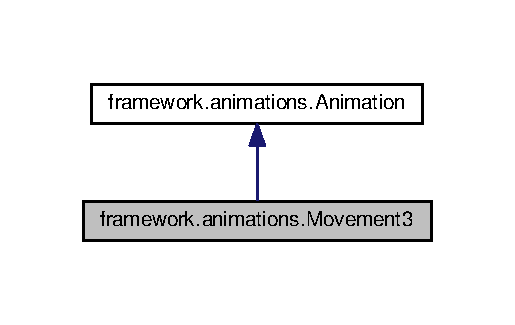
\includegraphics[width=247pt]{classframework_1_1animations_1_1Movement3__inherit__graph}
\end{center}
\end{figure}


Collaboration diagram for framework.\+animations.\+Movement3\+:
\nopagebreak
\begin{figure}[H]
\begin{center}
\leavevmode
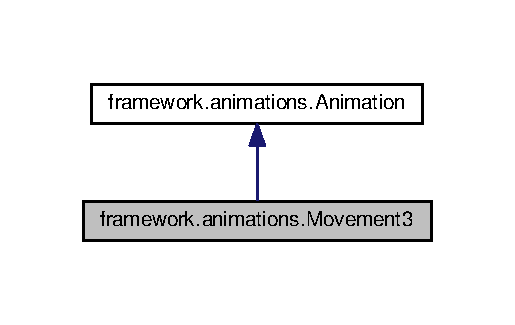
\includegraphics[width=247pt]{classframework_1_1animations_1_1Movement3__coll__graph}
\end{center}
\end{figure}
\subsection*{Public Member Functions}
\begin{DoxyCompactItemize}
\item 
def {\bfseries \+\_\+\+\_\+init\+\_\+\+\_\+} (self, bdr\+\_\+handler, blender\+\_\+object, frames)\hypertarget{classframework_1_1animations_1_1Movement3_ac45cdb928da0fa179c3465bc3225fbf3}{}\label{classframework_1_1animations_1_1Movement3_ac45cdb928da0fa179c3465bc3225fbf3}

\end{DoxyCompactItemize}
\subsection*{Static Public Member Functions}
\begin{DoxyCompactItemize}
\item 
def {\bfseries get\+\_\+start\+\_\+position} ()\hypertarget{classframework_1_1animations_1_1Movement3_afc96fbe112b3c4eef38de74a0bf89395}{}\label{classframework_1_1animations_1_1Movement3_afc96fbe112b3c4eef38de74a0bf89395}

\item 
def {\bfseries get\+\_\+start\+\_\+rotation} ()\hypertarget{classframework_1_1animations_1_1Movement3_ace7776473c907fb42291edaa5da914c4}{}\label{classframework_1_1animations_1_1Movement3_ace7776473c907fb42291edaa5da914c4}

\end{DoxyCompactItemize}
\subsection*{Static Public Attributes}
\begin{DoxyCompactItemize}
\item 
string {\bfseries interpolation} = \textquotesingle{}L\+I\+N\+E\+AR\textquotesingle{}\hypertarget{classframework_1_1animations_1_1Movement3_a1ae3a0543356314a3795e3c114c95797}{}\label{classframework_1_1animations_1_1Movement3_a1ae3a0543356314a3795e3c114c95797}

\end{DoxyCompactItemize}


The documentation for this class was generated from the following file\+:\begin{DoxyCompactItemize}
\item 
/home/sebastian/catkin\+\_\+ws/src/animation\+\_\+render/scripts/framework/animations.\+py\end{DoxyCompactItemize}

\hypertarget{classframework_1_1animations_1_1Movement4}{}\section{framework.\+animations.\+Movement4 Class Reference}
\label{classframework_1_1animations_1_1Movement4}\index{framework.\+animations.\+Movement4@{framework.\+animations.\+Movement4}}


Inheritance diagram for framework.\+animations.\+Movement4\+:
\nopagebreak
\begin{figure}[H]
\begin{center}
\leavevmode
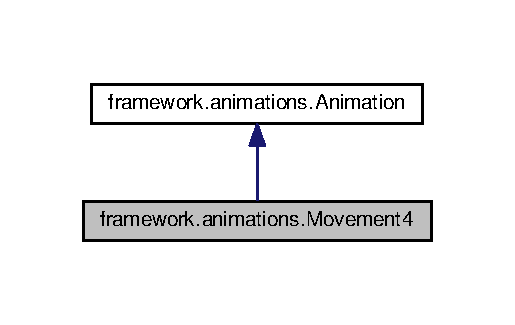
\includegraphics[width=247pt]{classframework_1_1animations_1_1Movement4__inherit__graph}
\end{center}
\end{figure}


Collaboration diagram for framework.\+animations.\+Movement4\+:
\nopagebreak
\begin{figure}[H]
\begin{center}
\leavevmode
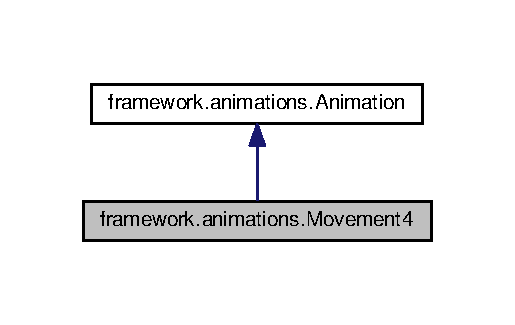
\includegraphics[width=247pt]{classframework_1_1animations_1_1Movement4__coll__graph}
\end{center}
\end{figure}
\subsection*{Public Member Functions}
\begin{DoxyCompactItemize}
\item 
def {\bfseries \+\_\+\+\_\+init\+\_\+\+\_\+} (self, bdr\+\_\+handler, blender\+\_\+object, frames)\hypertarget{classframework_1_1animations_1_1Movement4_a3f76014acac4b1078f20d08a91bc1260}{}\label{classframework_1_1animations_1_1Movement4_a3f76014acac4b1078f20d08a91bc1260}

\end{DoxyCompactItemize}
\subsection*{Static Public Member Functions}
\begin{DoxyCompactItemize}
\item 
def {\bfseries get\+\_\+start\+\_\+position} ()\hypertarget{classframework_1_1animations_1_1Movement4_aae872b08621755e27c97c1ae690762f2}{}\label{classframework_1_1animations_1_1Movement4_aae872b08621755e27c97c1ae690762f2}

\item 
def {\bfseries get\+\_\+start\+\_\+rotation} ()\hypertarget{classframework_1_1animations_1_1Movement4_a4dd4c7db340dad3435793401366c335a}{}\label{classframework_1_1animations_1_1Movement4_a4dd4c7db340dad3435793401366c335a}

\end{DoxyCompactItemize}
\subsection*{Static Public Attributes}
\begin{DoxyCompactItemize}
\item 
string {\bfseries interpolation} = \textquotesingle{}L\+I\+N\+E\+AR\textquotesingle{}\hypertarget{classframework_1_1animations_1_1Movement4_a0c7a1cb095e6aaff90318d164574f830}{}\label{classframework_1_1animations_1_1Movement4_a0c7a1cb095e6aaff90318d164574f830}

\end{DoxyCompactItemize}


The documentation for this class was generated from the following file\+:\begin{DoxyCompactItemize}
\item 
/home/sebastian/catkin\+\_\+ws/src/animation\+\_\+render/scripts/framework/animations.\+py\end{DoxyCompactItemize}

\hypertarget{classframework_1_1objects_1_1Plane}{}\section{framework.\+objects.\+Plane Class Reference}
\label{classframework_1_1objects_1_1Plane}\index{framework.\+objects.\+Plane@{framework.\+objects.\+Plane}}


Inheritance diagram for framework.\+objects.\+Plane\+:
\nopagebreak
\begin{figure}[H]
\begin{center}
\leavevmode
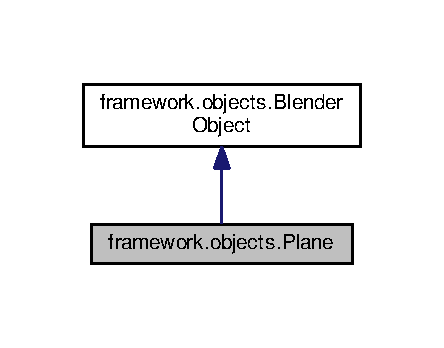
\includegraphics[width=213pt]{classframework_1_1objects_1_1Plane__inherit__graph}
\end{center}
\end{figure}


Collaboration diagram for framework.\+objects.\+Plane\+:
\nopagebreak
\begin{figure}[H]
\begin{center}
\leavevmode
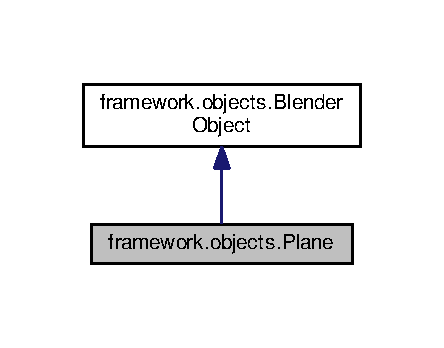
\includegraphics[width=213pt]{classframework_1_1objects_1_1Plane__coll__graph}
\end{center}
\end{figure}
\subsection*{Public Member Functions}
\begin{DoxyCompactItemize}
\item 
def {\bfseries \+\_\+\+\_\+init\+\_\+\+\_\+} (self, p1, p2, p3, image=None)\hypertarget{classframework_1_1objects_1_1Plane_abc66f95c67f305cfe51077ea7c75c221}{}\label{classframework_1_1objects_1_1Plane_abc66f95c67f305cfe51077ea7c75c221}

\end{DoxyCompactItemize}
\subsection*{Static Public Attributes}
\begin{DoxyCompactItemize}
\item 
{\bfseries width} = None\hypertarget{classframework_1_1objects_1_1Plane_a7e4a9b71e7e44d83075b37b97c980b52}{}\label{classframework_1_1objects_1_1Plane_a7e4a9b71e7e44d83075b37b97c980b52}

\item 
{\bfseries height} = None\hypertarget{classframework_1_1objects_1_1Plane_aca12d83777e52195580f6416b409d027}{}\label{classframework_1_1objects_1_1Plane_aca12d83777e52195580f6416b409d027}

\end{DoxyCompactItemize}


The documentation for this class was generated from the following file\+:\begin{DoxyCompactItemize}
\item 
/home/sebastian/catkin\+\_\+ws/src/animation\+\_\+render/scripts/framework/objects.\+py\end{DoxyCompactItemize}

\hypertarget{structPose}{}\section{Pose Struct Reference}
\label{structPose}\index{Pose@{Pose}}
\subsection*{Public Attributes}
\begin{DoxyCompactItemize}
\item 
double {\bfseries x}\hypertarget{structPose_a0061c7789df90f593ab95118cbef387f}{}\label{structPose_a0061c7789df90f593ab95118cbef387f}

\item 
double {\bfseries y}\hypertarget{structPose_a6280216efe0840a7a55f025ad04e3b3d}{}\label{structPose_a6280216efe0840a7a55f025ad04e3b3d}

\item 
double {\bfseries z}\hypertarget{structPose_ad92c1d2873955b2bed6b29ac984858c3}{}\label{structPose_ad92c1d2873955b2bed6b29ac984858c3}

\item 
double {\bfseries ax}\hypertarget{structPose_a1ea6c02833ae2ecdca4d11e9379138e6}{}\label{structPose_a1ea6c02833ae2ecdca4d11e9379138e6}

\item 
double {\bfseries ay}\hypertarget{structPose_a6e7e21014c615126b38e08657d350063}{}\label{structPose_a6e7e21014c615126b38e08657d350063}

\item 
double {\bfseries az}\hypertarget{structPose_a0ae7c9f223b181c09da2f07cae7842c3}{}\label{structPose_a0ae7c9f223b181c09da2f07cae7842c3}

\end{DoxyCompactItemize}


The documentation for this struct was generated from the following file\+:\begin{DoxyCompactItemize}
\item 
/home/sebastian/catkin\+\_\+ws/src/animation\+\_\+render/src/pythoncaller.\+h\end{DoxyCompactItemize}

\hypertarget{classPythonCaller}{}\section{Python\+Caller Class Reference}
\label{classPythonCaller}\index{Python\+Caller@{Python\+Caller}}
\subsection*{Public Member Functions}
\begin{DoxyCompactItemize}
\item 
{\bfseries Python\+Caller} (ros\+::\+Node\+Handle $\ast$nh)\hypertarget{classPythonCaller_a17b5967b8cb382fa420dee33870a186a}{}\label{classPythonCaller_a17b5967b8cb382fa420dee33870a186a}

\item 
void \hyperlink{classPythonCaller_a2f996721a3cddabbfb9181d826fc9335}{render\+Video} (std\+::string video\+\_\+name, std\+::string template\+\_\+name, std\+::string background\+\_\+name, \hyperlink{structVideoOptions}{Video\+Options} video\+\_\+options, std\+::string object, std\+::string animation, double mp1, double mp2, double mp3)
\begin{DoxyCompactList}\small\item\em Render video. \end{DoxyCompactList}\item 
void \hyperlink{classPythonCaller_a2edcddb9119570ee95b2f4fb6e18c58c}{get\+Image\+List} (std\+::string path, int length, int min\+\_\+height, int min\+\_\+width, std\+::string keywords)
\begin{DoxyCompactList}\small\item\em Creates a list of image urls. \end{DoxyCompactList}\item 
void \hyperlink{classPythonCaller_a6217d7fc3432b3464c274b3fe2c5c539}{download\+Image} (std\+::string filename, std\+::string list, int nr)
\begin{DoxyCompactList}\small\item\em Download image from list. \end{DoxyCompactList}\item 
void \hyperlink{classPythonCaller_a4a7706b979cfe9aa45f1dcbc80d9a942}{get\+Ground\+Truth\+Data} (std\+::string animation, int frames, std\+::string path)
\begin{DoxyCompactList}\small\item\em Get the ground truth data of given animation. \end{DoxyCompactList}\item 
void \hyperlink{classPythonCaller_a690a2ad68abc1dc354eb74b9c58e65e7}{get\+Init\+Pose} (std\+::string animation, \hyperlink{structPose}{Pose} \&init\+Pose)
\begin{DoxyCompactList}\small\item\em Get init pose of animation. \end{DoxyCompactList}\end{DoxyCompactItemize}


\subsection{Member Function Documentation}
\index{Python\+Caller@{Python\+Caller}!download\+Image@{download\+Image}}
\index{download\+Image@{download\+Image}!Python\+Caller@{Python\+Caller}}
\subsubsection[{\texorpdfstring{download\+Image(std\+::string filename, std\+::string list, int nr)}{downloadImage(std::string filename, std::string list, int nr)}}]{\setlength{\rightskip}{0pt plus 5cm}void Python\+Caller\+::download\+Image (
\begin{DoxyParamCaption}
\item[{std\+::string}]{filename, }
\item[{std\+::string}]{list, }
\item[{int}]{nr}
\end{DoxyParamCaption}
)}\hypertarget{classPythonCaller_a6217d7fc3432b3464c274b3fe2c5c539}{}\label{classPythonCaller_a6217d7fc3432b3464c274b3fe2c5c539}


Download image from list. 


\begin{DoxyParams}{Parameters}
{\em nr} & Index of image \\
\hline
\end{DoxyParams}
\index{Python\+Caller@{Python\+Caller}!get\+Ground\+Truth\+Data@{get\+Ground\+Truth\+Data}}
\index{get\+Ground\+Truth\+Data@{get\+Ground\+Truth\+Data}!Python\+Caller@{Python\+Caller}}
\subsubsection[{\texorpdfstring{get\+Ground\+Truth\+Data(std\+::string animation, int frames, std\+::string path)}{getGroundTruthData(std::string animation, int frames, std::string path)}}]{\setlength{\rightskip}{0pt plus 5cm}void Python\+Caller\+::get\+Ground\+Truth\+Data (
\begin{DoxyParamCaption}
\item[{std\+::string}]{animation, }
\item[{int}]{frames, }
\item[{std\+::string}]{path}
\end{DoxyParamCaption}
)}\hypertarget{classPythonCaller_a4a7706b979cfe9aa45f1dcbc80d9a942}{}\label{classPythonCaller_a4a7706b979cfe9aa45f1dcbc80d9a942}


Get the ground truth data of given animation. 


\begin{DoxyParams}{Parameters}
{\em animation} & Name of animation \\
\hline
{\em frames} & Number of frames \\
\hline
{\em path} & output path \\
\hline
\end{DoxyParams}
\index{Python\+Caller@{Python\+Caller}!get\+Image\+List@{get\+Image\+List}}
\index{get\+Image\+List@{get\+Image\+List}!Python\+Caller@{Python\+Caller}}
\subsubsection[{\texorpdfstring{get\+Image\+List(std\+::string path, int length, int min\+\_\+height, int min\+\_\+width, std\+::string keywords)}{getImageList(std::string path, int length, int min_height, int min_width, std::string keywords)}}]{\setlength{\rightskip}{0pt plus 5cm}void Python\+Caller\+::get\+Image\+List (
\begin{DoxyParamCaption}
\item[{std\+::string}]{path, }
\item[{int}]{length, }
\item[{int}]{min\+\_\+height, }
\item[{int}]{min\+\_\+width, }
\item[{std\+::string}]{keywords}
\end{DoxyParamCaption}
)}\hypertarget{classPythonCaller_a2edcddb9119570ee95b2f4fb6e18c58c}{}\label{classPythonCaller_a2edcddb9119570ee95b2f4fb6e18c58c}


Creates a list of image urls. 


\begin{DoxyParams}{Parameters}
{\em length} & Length of list \\
\hline
{\em min\+\_\+height} & Minimal height of images \\
\hline
{\em min\+\_\+width} & Minimal width of images \\
\hline
{\em keywords} & Some keywords to search for \\
\hline
\end{DoxyParams}
\index{Python\+Caller@{Python\+Caller}!get\+Init\+Pose@{get\+Init\+Pose}}
\index{get\+Init\+Pose@{get\+Init\+Pose}!Python\+Caller@{Python\+Caller}}
\subsubsection[{\texorpdfstring{get\+Init\+Pose(std\+::string animation, Pose \&init\+Pose)}{getInitPose(std::string animation, Pose &initPose)}}]{\setlength{\rightskip}{0pt plus 5cm}void Python\+Caller\+::get\+Init\+Pose (
\begin{DoxyParamCaption}
\item[{std\+::string}]{animation, }
\item[{{\bf Pose} \&}]{init\+Pose}
\end{DoxyParamCaption}
)}\hypertarget{classPythonCaller_a690a2ad68abc1dc354eb74b9c58e65e7}{}\label{classPythonCaller_a690a2ad68abc1dc354eb74b9c58e65e7}


Get init pose of animation. 


\begin{DoxyParams}{Parameters}
{\em animation} & Name of animation \\
\hline
{\em x} & x position \\
\hline
{\em y} & y position \\
\hline
{\em z} & z position \\
\hline
{\em ax} & angle x \\
\hline
{\em ay} & angle y \\
\hline
{\em az} & angle z \\
\hline
\end{DoxyParams}
\index{Python\+Caller@{Python\+Caller}!render\+Video@{render\+Video}}
\index{render\+Video@{render\+Video}!Python\+Caller@{Python\+Caller}}
\subsubsection[{\texorpdfstring{render\+Video(std\+::string video\+\_\+name, std\+::string template\+\_\+name, std\+::string background\+\_\+name, Video\+Options video\+\_\+options, std\+::string object, std\+::string animation, double mp1, double mp2, double mp3)}{renderVideo(std::string video_name, std::string template_name, std::string background_name, VideoOptions video_options, std::string object, std::string animation, double mp1, double mp2, double mp3)}}]{\setlength{\rightskip}{0pt plus 5cm}void Python\+Caller\+::render\+Video (
\begin{DoxyParamCaption}
\item[{std\+::string}]{video\+\_\+name, }
\item[{std\+::string}]{template\+\_\+name, }
\item[{std\+::string}]{background\+\_\+name, }
\item[{{\bf Video\+Options}}]{video\+\_\+options, }
\item[{std\+::string}]{object, }
\item[{std\+::string}]{animation, }
\item[{double}]{mp1, }
\item[{double}]{mp2, }
\item[{double}]{mp3}
\end{DoxyParamCaption}
)}\hypertarget{classPythonCaller_a2f996721a3cddabbfb9181d826fc9335}{}\label{classPythonCaller_a2f996721a3cddabbfb9181d826fc9335}


Render video. 


\begin{DoxyParams}{Parameters}
{\em frames} & Number frames \\
\hline
{\em fps} & Frames per second \\
\hline
{\em object} & Name of object\+: Plane, Cylinder \\
\hline
{\em animation} & Name of animation \\
\hline
{\em res\+\_\+x} & Resolution x \\
\hline
{\em res\+\_\+y} & Resolution y \\
\hline
{\em mp1} & Model parameter 1 \\
\hline
{\em mp2} & Model parameter 2 \\
\hline
{\em mp3} & Model parameter 3 \\
\hline
\end{DoxyParams}


The documentation for this class was generated from the following files\+:\begin{DoxyCompactItemize}
\item 
/home/sebastian/catkin\+\_\+ws/src/animation\+\_\+render/src/pythoncaller.\+h\item 
/home/sebastian/catkin\+\_\+ws/src/animation\+\_\+render/src/pythoncaller.\+cpp\end{DoxyCompactItemize}

\hypertarget{classframework_1_1animations_1_1RandomMixed}{}\section{framework.\+animations.\+Random\+Mixed Class Reference}
\label{classframework_1_1animations_1_1RandomMixed}\index{framework.\+animations.\+Random\+Mixed@{framework.\+animations.\+Random\+Mixed}}


Inheritance diagram for framework.\+animations.\+Random\+Mixed\+:
\nopagebreak
\begin{figure}[H]
\begin{center}
\leavevmode
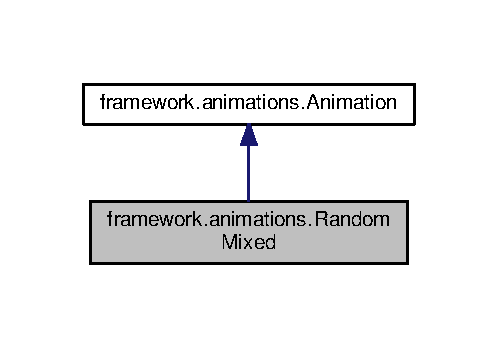
\includegraphics[width=239pt]{classframework_1_1animations_1_1RandomMixed__inherit__graph}
\end{center}
\end{figure}


Collaboration diagram for framework.\+animations.\+Random\+Mixed\+:
\nopagebreak
\begin{figure}[H]
\begin{center}
\leavevmode
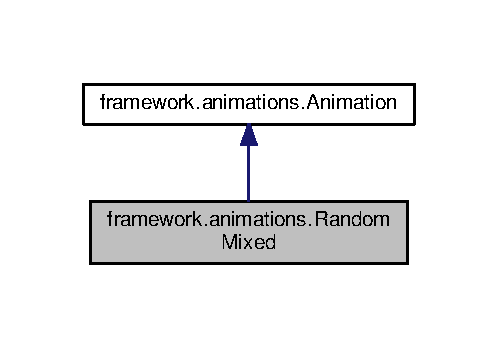
\includegraphics[width=239pt]{classframework_1_1animations_1_1RandomMixed__coll__graph}
\end{center}
\end{figure}
\subsection*{Public Member Functions}
\begin{DoxyCompactItemize}
\item 
def {\bfseries \+\_\+\+\_\+init\+\_\+\+\_\+} (self, bdr\+\_\+handler, blender\+\_\+object, frames)\hypertarget{classframework_1_1animations_1_1RandomMixed_aca5bef51a8fa5a084208e58a45565cbd}{}\label{classframework_1_1animations_1_1RandomMixed_aca5bef51a8fa5a084208e58a45565cbd}

\end{DoxyCompactItemize}
\subsection*{Static Public Member Functions}
\begin{DoxyCompactItemize}
\item 
def {\bfseries get\+\_\+start\+\_\+position} ()\hypertarget{classframework_1_1animations_1_1RandomMixed_a971cba1d986fa01e2fe3fc01bb6e0ddd}{}\label{classframework_1_1animations_1_1RandomMixed_a971cba1d986fa01e2fe3fc01bb6e0ddd}

\item 
def {\bfseries get\+\_\+start\+\_\+rotation} ()\hypertarget{classframework_1_1animations_1_1RandomMixed_a2a8ab0ae8b96b85fd7621813aeee3ecd}{}\label{classframework_1_1animations_1_1RandomMixed_a2a8ab0ae8b96b85fd7621813aeee3ecd}

\end{DoxyCompactItemize}
\subsection*{Static Public Attributes}
\begin{DoxyCompactItemize}
\item 
string {\bfseries interpolation} = \textquotesingle{}L\+I\+N\+E\+AR\textquotesingle{}\hypertarget{classframework_1_1animations_1_1RandomMixed_a6c109d99d37a18dd808c79d4d4e7e37f}{}\label{classframework_1_1animations_1_1RandomMixed_a6c109d99d37a18dd808c79d4d4e7e37f}

\end{DoxyCompactItemize}


The documentation for this class was generated from the following file\+:\begin{DoxyCompactItemize}
\item 
/home/sebastian/catkin\+\_\+ws/src/animation\+\_\+render/scripts/framework/animations.\+py\end{DoxyCompactItemize}

\hypertarget{classframework_1_1animations_1_1RandomMovement}{}\section{framework.\+animations.\+Random\+Movement Class Reference}
\label{classframework_1_1animations_1_1RandomMovement}\index{framework.\+animations.\+Random\+Movement@{framework.\+animations.\+Random\+Movement}}


Inheritance diagram for framework.\+animations.\+Random\+Movement\+:
\nopagebreak
\begin{figure}[H]
\begin{center}
\leavevmode
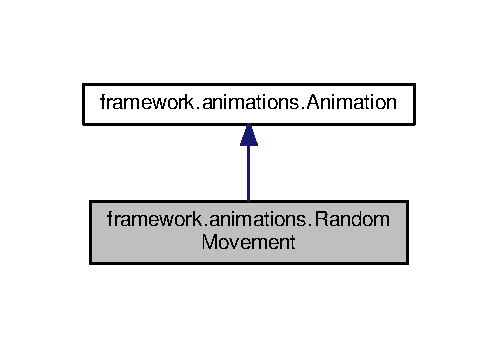
\includegraphics[width=239pt]{classframework_1_1animations_1_1RandomMovement__inherit__graph}
\end{center}
\end{figure}


Collaboration diagram for framework.\+animations.\+Random\+Movement\+:
\nopagebreak
\begin{figure}[H]
\begin{center}
\leavevmode
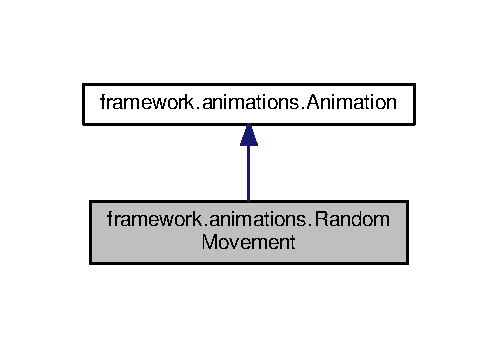
\includegraphics[width=239pt]{classframework_1_1animations_1_1RandomMovement__coll__graph}
\end{center}
\end{figure}
\subsection*{Public Member Functions}
\begin{DoxyCompactItemize}
\item 
def {\bfseries \+\_\+\+\_\+init\+\_\+\+\_\+} (self, bdr\+\_\+handler, blender\+\_\+object, frames)\hypertarget{classframework_1_1animations_1_1RandomMovement_a8af0da4ac19f03fc9a61063cd92ad7b7}{}\label{classframework_1_1animations_1_1RandomMovement_a8af0da4ac19f03fc9a61063cd92ad7b7}

\end{DoxyCompactItemize}
\subsection*{Static Public Member Functions}
\begin{DoxyCompactItemize}
\item 
def {\bfseries get\+\_\+start\+\_\+position} ()\hypertarget{classframework_1_1animations_1_1RandomMovement_a26672551cfe2bb0f7c38cd0e716c2dd2}{}\label{classframework_1_1animations_1_1RandomMovement_a26672551cfe2bb0f7c38cd0e716c2dd2}

\item 
def {\bfseries get\+\_\+start\+\_\+rotation} ()\hypertarget{classframework_1_1animations_1_1RandomMovement_a94f2b948a4538f6e86bd2ddc2c7bf59e}{}\label{classframework_1_1animations_1_1RandomMovement_a94f2b948a4538f6e86bd2ddc2c7bf59e}

\end{DoxyCompactItemize}
\subsection*{Static Public Attributes}
\begin{DoxyCompactItemize}
\item 
string {\bfseries interpolation} = \textquotesingle{}L\+I\+N\+E\+AR\textquotesingle{}\hypertarget{classframework_1_1animations_1_1RandomMovement_ab1271d0ddc9bd00ec975b886da8f1c07}{}\label{classframework_1_1animations_1_1RandomMovement_ab1271d0ddc9bd00ec975b886da8f1c07}

\end{DoxyCompactItemize}


The documentation for this class was generated from the following file\+:\begin{DoxyCompactItemize}
\item 
/home/sebastian/catkin\+\_\+ws/src/animation\+\_\+render/scripts/framework/animations.\+py\end{DoxyCompactItemize}

\hypertarget{classframework_1_1animations_1_1RandomRotation}{}\section{framework.\+animations.\+Random\+Rotation Class Reference}
\label{classframework_1_1animations_1_1RandomRotation}\index{framework.\+animations.\+Random\+Rotation@{framework.\+animations.\+Random\+Rotation}}


Inheritance diagram for framework.\+animations.\+Random\+Rotation\+:
\nopagebreak
\begin{figure}[H]
\begin{center}
\leavevmode
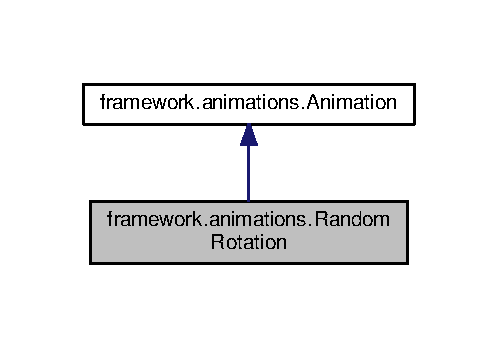
\includegraphics[width=239pt]{classframework_1_1animations_1_1RandomRotation__inherit__graph}
\end{center}
\end{figure}


Collaboration diagram for framework.\+animations.\+Random\+Rotation\+:
\nopagebreak
\begin{figure}[H]
\begin{center}
\leavevmode
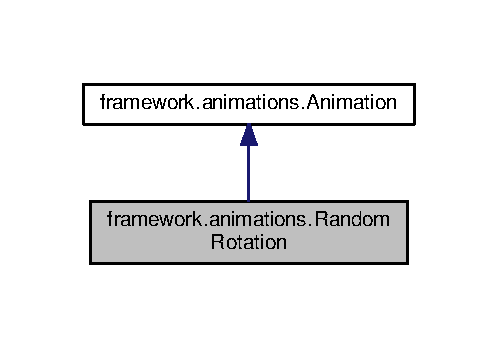
\includegraphics[width=239pt]{classframework_1_1animations_1_1RandomRotation__coll__graph}
\end{center}
\end{figure}
\subsection*{Public Member Functions}
\begin{DoxyCompactItemize}
\item 
def {\bfseries \+\_\+\+\_\+init\+\_\+\+\_\+} (self, bdr\+\_\+handler, blender\+\_\+object, frames)\hypertarget{classframework_1_1animations_1_1RandomRotation_a095a809c807ec64f927e4370b712ff9e}{}\label{classframework_1_1animations_1_1RandomRotation_a095a809c807ec64f927e4370b712ff9e}

\end{DoxyCompactItemize}
\subsection*{Static Public Member Functions}
\begin{DoxyCompactItemize}
\item 
def {\bfseries get\+\_\+start\+\_\+position} ()\hypertarget{classframework_1_1animations_1_1RandomRotation_ad26e308593e71b663bb0d929ea0bb5c7}{}\label{classframework_1_1animations_1_1RandomRotation_ad26e308593e71b663bb0d929ea0bb5c7}

\item 
def {\bfseries get\+\_\+start\+\_\+rotation} ()\hypertarget{classframework_1_1animations_1_1RandomRotation_a7408abc3d3579b28408082ee984c2ba7}{}\label{classframework_1_1animations_1_1RandomRotation_a7408abc3d3579b28408082ee984c2ba7}

\end{DoxyCompactItemize}
\subsection*{Static Public Attributes}
\begin{DoxyCompactItemize}
\item 
string {\bfseries interpolation} = \textquotesingle{}L\+I\+N\+E\+AR\textquotesingle{}\hypertarget{classframework_1_1animations_1_1RandomRotation_aae12370812df296572b2b11752e02329}{}\label{classframework_1_1animations_1_1RandomRotation_aae12370812df296572b2b11752e02329}

\end{DoxyCompactItemize}


The documentation for this class was generated from the following file\+:\begin{DoxyCompactItemize}
\item 
/home/sebastian/catkin\+\_\+ws/src/animation\+\_\+render/scripts/framework/animations.\+py\end{DoxyCompactItemize}

\hypertarget{classframework_1_1animations_1_1RenderTest}{}\section{framework.\+animations.\+Render\+Test Class Reference}
\label{classframework_1_1animations_1_1RenderTest}\index{framework.\+animations.\+Render\+Test@{framework.\+animations.\+Render\+Test}}


Inheritance diagram for framework.\+animations.\+Render\+Test\+:
\nopagebreak
\begin{figure}[H]
\begin{center}
\leavevmode
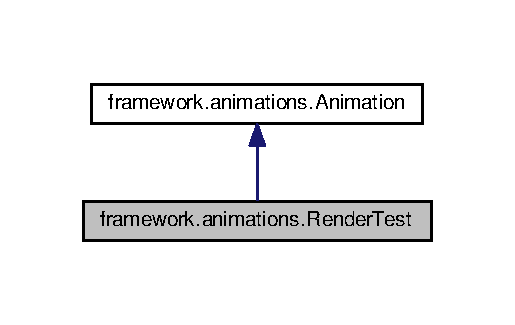
\includegraphics[width=247pt]{classframework_1_1animations_1_1RenderTest__inherit__graph}
\end{center}
\end{figure}


Collaboration diagram for framework.\+animations.\+Render\+Test\+:
\nopagebreak
\begin{figure}[H]
\begin{center}
\leavevmode
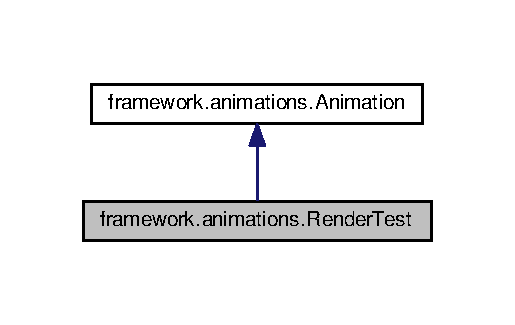
\includegraphics[width=247pt]{classframework_1_1animations_1_1RenderTest__coll__graph}
\end{center}
\end{figure}
\subsection*{Public Member Functions}
\begin{DoxyCompactItemize}
\item 
def {\bfseries \+\_\+\+\_\+init\+\_\+\+\_\+} (self, bdr\+\_\+handler, blender\+\_\+object, frames)\hypertarget{classframework_1_1animations_1_1RenderTest_aa88a2318c3c4e47be17feb86c3a94514}{}\label{classframework_1_1animations_1_1RenderTest_aa88a2318c3c4e47be17feb86c3a94514}

\end{DoxyCompactItemize}
\subsection*{Static Public Member Functions}
\begin{DoxyCompactItemize}
\item 
def {\bfseries get\+\_\+start\+\_\+position} ()\hypertarget{classframework_1_1animations_1_1RenderTest_a9493aa8ac3dcc53f14e010c06e6799fd}{}\label{classframework_1_1animations_1_1RenderTest_a9493aa8ac3dcc53f14e010c06e6799fd}

\item 
def {\bfseries get\+\_\+start\+\_\+rotation} ()\hypertarget{classframework_1_1animations_1_1RenderTest_ad88b577b9a8741e3cb0ce1c235c031e2}{}\label{classframework_1_1animations_1_1RenderTest_ad88b577b9a8741e3cb0ce1c235c031e2}

\end{DoxyCompactItemize}
\subsection*{Additional Inherited Members}


The documentation for this class was generated from the following file\+:\begin{DoxyCompactItemize}
\item 
/home/sebastian/catkin\+\_\+ws/src/animation\+\_\+render/scripts/framework/animations.\+py\end{DoxyCompactItemize}

\hypertarget{classframework_1_1animations_1_1RotationX}{}\section{framework.\+animations.\+RotationX Class Reference}
\label{classframework_1_1animations_1_1RotationX}\index{framework.\+animations.\+RotationX@{framework.\+animations.\+RotationX}}


Inheritance diagram for framework.\+animations.\+RotationX\+:
\nopagebreak
\begin{figure}[H]
\begin{center}
\leavevmode
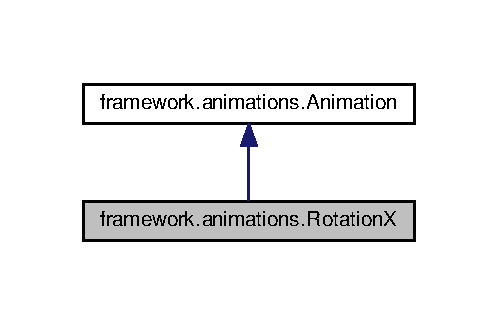
\includegraphics[width=239pt]{classframework_1_1animations_1_1RotationX__inherit__graph}
\end{center}
\end{figure}


Collaboration diagram for framework.\+animations.\+RotationX\+:
\nopagebreak
\begin{figure}[H]
\begin{center}
\leavevmode
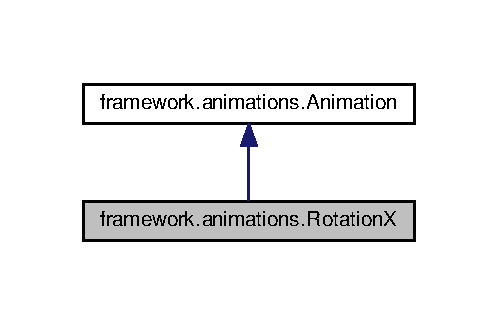
\includegraphics[width=239pt]{classframework_1_1animations_1_1RotationX__coll__graph}
\end{center}
\end{figure}
\subsection*{Public Member Functions}
\begin{DoxyCompactItemize}
\item 
def {\bfseries \+\_\+\+\_\+init\+\_\+\+\_\+} (self, bdr\+\_\+handler, blender\+\_\+object, frames)\hypertarget{classframework_1_1animations_1_1RotationX_ab2109fd69ef8a189f9d4b062fb6825f3}{}\label{classframework_1_1animations_1_1RotationX_ab2109fd69ef8a189f9d4b062fb6825f3}

\end{DoxyCompactItemize}
\subsection*{Static Public Member Functions}
\begin{DoxyCompactItemize}
\item 
def {\bfseries get\+\_\+start\+\_\+position} ()\hypertarget{classframework_1_1animations_1_1RotationX_a5a868f5d5e4d0ac36a2d00ed12068c45}{}\label{classframework_1_1animations_1_1RotationX_a5a868f5d5e4d0ac36a2d00ed12068c45}

\item 
def {\bfseries get\+\_\+start\+\_\+rotation} ()\hypertarget{classframework_1_1animations_1_1RotationX_a325b094da99e82ca13d74a25323fe60d}{}\label{classframework_1_1animations_1_1RotationX_a325b094da99e82ca13d74a25323fe60d}

\end{DoxyCompactItemize}
\subsection*{Static Public Attributes}
\begin{DoxyCompactItemize}
\item 
string {\bfseries interpolation} = \textquotesingle{}Q\+U\+AD\textquotesingle{}\hypertarget{classframework_1_1animations_1_1RotationX_a48c000cbff8dc78c4be96decdae00405}{}\label{classframework_1_1animations_1_1RotationX_a48c000cbff8dc78c4be96decdae00405}

\end{DoxyCompactItemize}


The documentation for this class was generated from the following file\+:\begin{DoxyCompactItemize}
\item 
/home/sebastian/catkin\+\_\+ws/src/animation\+\_\+render/scripts/framework/animations.\+py\end{DoxyCompactItemize}

\hypertarget{classframework_1_1animations_1_1RotationX2}{}\section{framework.\+animations.\+Rotation\+X2 Class Reference}
\label{classframework_1_1animations_1_1RotationX2}\index{framework.\+animations.\+Rotation\+X2@{framework.\+animations.\+Rotation\+X2}}


Inheritance diagram for framework.\+animations.\+Rotation\+X2\+:
\nopagebreak
\begin{figure}[H]
\begin{center}
\leavevmode
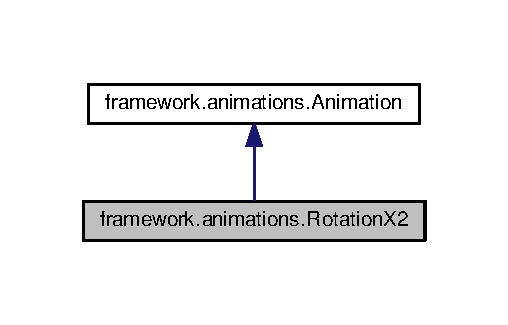
\includegraphics[width=244pt]{classframework_1_1animations_1_1RotationX2__inherit__graph}
\end{center}
\end{figure}


Collaboration diagram for framework.\+animations.\+Rotation\+X2\+:
\nopagebreak
\begin{figure}[H]
\begin{center}
\leavevmode
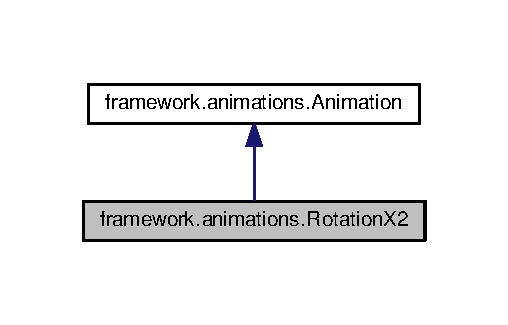
\includegraphics[width=244pt]{classframework_1_1animations_1_1RotationX2__coll__graph}
\end{center}
\end{figure}
\subsection*{Public Member Functions}
\begin{DoxyCompactItemize}
\item 
def {\bfseries \+\_\+\+\_\+init\+\_\+\+\_\+} (self, bdr\+\_\+handler, blender\+\_\+object, frames)\hypertarget{classframework_1_1animations_1_1RotationX2_a4c9bbc3d03d5976a48d9ce9ab6539600}{}\label{classframework_1_1animations_1_1RotationX2_a4c9bbc3d03d5976a48d9ce9ab6539600}

\end{DoxyCompactItemize}
\subsection*{Static Public Member Functions}
\begin{DoxyCompactItemize}
\item 
def {\bfseries get\+\_\+start\+\_\+position} ()\hypertarget{classframework_1_1animations_1_1RotationX2_a1cbd524eed28fd0b5e51e59996f05dec}{}\label{classframework_1_1animations_1_1RotationX2_a1cbd524eed28fd0b5e51e59996f05dec}

\item 
def {\bfseries get\+\_\+start\+\_\+rotation} ()\hypertarget{classframework_1_1animations_1_1RotationX2_ab6c032accf0217aea8676a2017779c96}{}\label{classframework_1_1animations_1_1RotationX2_ab6c032accf0217aea8676a2017779c96}

\end{DoxyCompactItemize}
\subsection*{Static Public Attributes}
\begin{DoxyCompactItemize}
\item 
string {\bfseries interpolation} = \textquotesingle{}Q\+U\+AD\textquotesingle{}\hypertarget{classframework_1_1animations_1_1RotationX2_a421dc124d8e2c0fcdf33c14665be0353}{}\label{classframework_1_1animations_1_1RotationX2_a421dc124d8e2c0fcdf33c14665be0353}

\end{DoxyCompactItemize}


The documentation for this class was generated from the following file\+:\begin{DoxyCompactItemize}
\item 
/home/sebastian/catkin\+\_\+ws/src/animation\+\_\+render/scripts/framework/animations.\+py\end{DoxyCompactItemize}

\hypertarget{classframework_1_1animations_1_1RotationXacc}{}\section{framework.\+animations.\+Rotation\+Xacc Class Reference}
\label{classframework_1_1animations_1_1RotationXacc}\index{framework.\+animations.\+Rotation\+Xacc@{framework.\+animations.\+Rotation\+Xacc}}


Inheritance diagram for framework.\+animations.\+Rotation\+Xacc\+:
\nopagebreak
\begin{figure}[H]
\begin{center}
\leavevmode
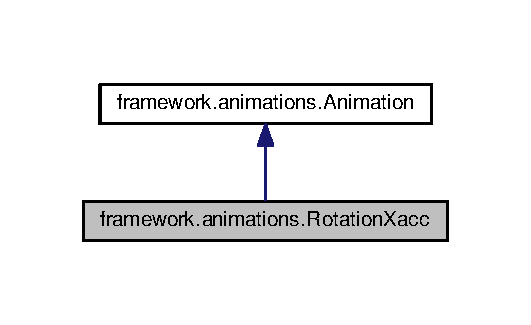
\includegraphics[width=255pt]{classframework_1_1animations_1_1RotationXacc__inherit__graph}
\end{center}
\end{figure}


Collaboration diagram for framework.\+animations.\+Rotation\+Xacc\+:
\nopagebreak
\begin{figure}[H]
\begin{center}
\leavevmode
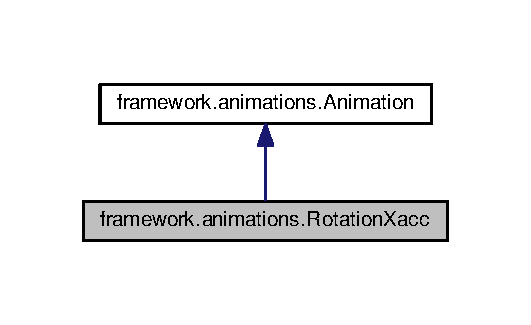
\includegraphics[width=255pt]{classframework_1_1animations_1_1RotationXacc__coll__graph}
\end{center}
\end{figure}
\subsection*{Public Member Functions}
\begin{DoxyCompactItemize}
\item 
def {\bfseries \+\_\+\+\_\+init\+\_\+\+\_\+} (self, bdr\+\_\+handler, blender\+\_\+object, frames)\hypertarget{classframework_1_1animations_1_1RotationXacc_ad2b45d8165a966b0ea12db042d346ae3}{}\label{classframework_1_1animations_1_1RotationXacc_ad2b45d8165a966b0ea12db042d346ae3}

\end{DoxyCompactItemize}
\subsection*{Static Public Member Functions}
\begin{DoxyCompactItemize}
\item 
def {\bfseries get\+\_\+start\+\_\+position} ()\hypertarget{classframework_1_1animations_1_1RotationXacc_a1aeb89f1baeef16e84414ad55df33ca1}{}\label{classframework_1_1animations_1_1RotationXacc_a1aeb89f1baeef16e84414ad55df33ca1}

\item 
def {\bfseries get\+\_\+start\+\_\+rotation} ()\hypertarget{classframework_1_1animations_1_1RotationXacc_a41156e7b6843acef1d061f1e3fd14df2}{}\label{classframework_1_1animations_1_1RotationXacc_a41156e7b6843acef1d061f1e3fd14df2}

\end{DoxyCompactItemize}
\subsection*{Static Public Attributes}
\begin{DoxyCompactItemize}
\item 
string {\bfseries interpolation} = \textquotesingle{}Q\+U\+AD\textquotesingle{}\hypertarget{classframework_1_1animations_1_1RotationXacc_aaca28e49c34d474cf88c1314040ebad5}{}\label{classframework_1_1animations_1_1RotationXacc_aaca28e49c34d474cf88c1314040ebad5}

\end{DoxyCompactItemize}


The documentation for this class was generated from the following file\+:\begin{DoxyCompactItemize}
\item 
/home/sebastian/catkin\+\_\+ws/src/animation\+\_\+render/scripts/framework/animations.\+py\end{DoxyCompactItemize}

\hypertarget{classframework_1_1animations_1_1RotationY}{}\section{framework.\+animations.\+RotationY Class Reference}
\label{classframework_1_1animations_1_1RotationY}\index{framework.\+animations.\+RotationY@{framework.\+animations.\+RotationY}}


Inheritance diagram for framework.\+animations.\+RotationY\+:
\nopagebreak
\begin{figure}[H]
\begin{center}
\leavevmode
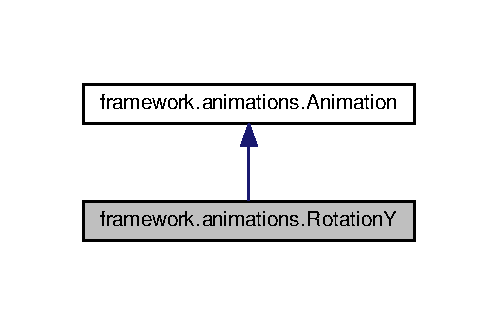
\includegraphics[width=239pt]{classframework_1_1animations_1_1RotationY__inherit__graph}
\end{center}
\end{figure}


Collaboration diagram for framework.\+animations.\+RotationY\+:
\nopagebreak
\begin{figure}[H]
\begin{center}
\leavevmode
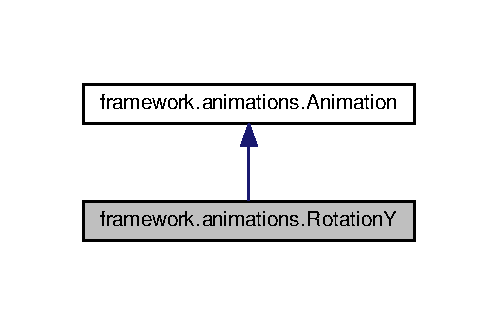
\includegraphics[width=239pt]{classframework_1_1animations_1_1RotationY__coll__graph}
\end{center}
\end{figure}
\subsection*{Public Member Functions}
\begin{DoxyCompactItemize}
\item 
def {\bfseries \+\_\+\+\_\+init\+\_\+\+\_\+} (self, bdr\+\_\+handler, blender\+\_\+object, frames)\hypertarget{classframework_1_1animations_1_1RotationY_acc35ac30c5b05ed6b40921ef5faba1a5}{}\label{classframework_1_1animations_1_1RotationY_acc35ac30c5b05ed6b40921ef5faba1a5}

\end{DoxyCompactItemize}
\subsection*{Static Public Member Functions}
\begin{DoxyCompactItemize}
\item 
def {\bfseries get\+\_\+start\+\_\+position} ()\hypertarget{classframework_1_1animations_1_1RotationY_aa8e3c7599aa32b7e74485f2f3493276f}{}\label{classframework_1_1animations_1_1RotationY_aa8e3c7599aa32b7e74485f2f3493276f}

\item 
def {\bfseries get\+\_\+start\+\_\+rotation} ()\hypertarget{classframework_1_1animations_1_1RotationY_a3941f53c4ec62340b217b4dd0a266ffd}{}\label{classframework_1_1animations_1_1RotationY_a3941f53c4ec62340b217b4dd0a266ffd}

\end{DoxyCompactItemize}
\subsection*{Static Public Attributes}
\begin{DoxyCompactItemize}
\item 
string {\bfseries interpolation} = \textquotesingle{}L\+I\+N\+E\+AR\textquotesingle{}\hypertarget{classframework_1_1animations_1_1RotationY_a288b9663c4bc34d2398c7fe5d648e9a0}{}\label{classframework_1_1animations_1_1RotationY_a288b9663c4bc34d2398c7fe5d648e9a0}

\end{DoxyCompactItemize}


The documentation for this class was generated from the following file\+:\begin{DoxyCompactItemize}
\item 
/home/sebastian/catkin\+\_\+ws/src/animation\+\_\+render/scripts/framework/animations.\+py\end{DoxyCompactItemize}

\hypertarget{classframework_1_1animations_1_1RotationZ}{}\section{framework.\+animations.\+RotationZ Class Reference}
\label{classframework_1_1animations_1_1RotationZ}\index{framework.\+animations.\+RotationZ@{framework.\+animations.\+RotationZ}}


Inheritance diagram for framework.\+animations.\+RotationZ\+:
\nopagebreak
\begin{figure}[H]
\begin{center}
\leavevmode
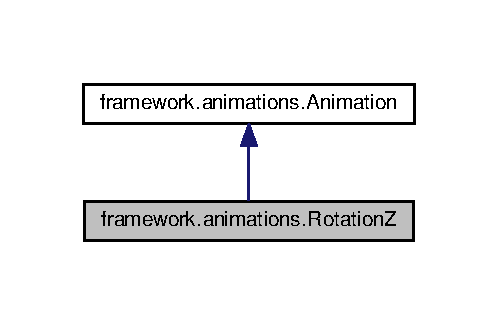
\includegraphics[width=239pt]{classframework_1_1animations_1_1RotationZ__inherit__graph}
\end{center}
\end{figure}


Collaboration diagram for framework.\+animations.\+RotationZ\+:
\nopagebreak
\begin{figure}[H]
\begin{center}
\leavevmode
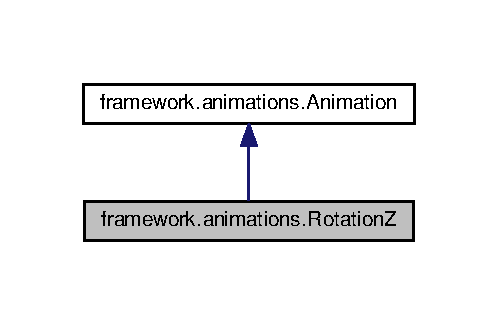
\includegraphics[width=239pt]{classframework_1_1animations_1_1RotationZ__coll__graph}
\end{center}
\end{figure}
\subsection*{Public Member Functions}
\begin{DoxyCompactItemize}
\item 
def {\bfseries \+\_\+\+\_\+init\+\_\+\+\_\+} (self, bdr\+\_\+handler, blender\+\_\+object, frames)\hypertarget{classframework_1_1animations_1_1RotationZ_ae7dd9ed1b41c74b9b5d26e29e9cc6600}{}\label{classframework_1_1animations_1_1RotationZ_ae7dd9ed1b41c74b9b5d26e29e9cc6600}

\end{DoxyCompactItemize}
\subsection*{Static Public Member Functions}
\begin{DoxyCompactItemize}
\item 
def {\bfseries get\+\_\+start\+\_\+position} ()\hypertarget{classframework_1_1animations_1_1RotationZ_ae9df85c778da7c7c77c7238666fa0036}{}\label{classframework_1_1animations_1_1RotationZ_ae9df85c778da7c7c77c7238666fa0036}

\item 
def {\bfseries get\+\_\+start\+\_\+rotation} ()\hypertarget{classframework_1_1animations_1_1RotationZ_a467180d7106f0877b9044ad2f99d9058}{}\label{classframework_1_1animations_1_1RotationZ_a467180d7106f0877b9044ad2f99d9058}

\end{DoxyCompactItemize}
\subsection*{Static Public Attributes}
\begin{DoxyCompactItemize}
\item 
string {\bfseries interpolation} = \textquotesingle{}Q\+U\+AD\textquotesingle{}\hypertarget{classframework_1_1animations_1_1RotationZ_a0a01f9bffae27973e7bedac463a45e53}{}\label{classframework_1_1animations_1_1RotationZ_a0a01f9bffae27973e7bedac463a45e53}

\end{DoxyCompactItemize}


The documentation for this class was generated from the following file\+:\begin{DoxyCompactItemize}
\item 
/home/sebastian/catkin\+\_\+ws/src/animation\+\_\+render/scripts/framework/animations.\+py\end{DoxyCompactItemize}

\hypertarget{classTemplateEvaluation}{}\section{Template\+Evaluation Class Reference}
\label{classTemplateEvaluation}\index{Template\+Evaluation@{Template\+Evaluation}}
\subsection*{Public Member Functions}
\begin{DoxyCompactItemize}
\item 
{\bfseries Template\+Evaluation} (double t\+\_\+grad, double t\+\_\+acc)\hypertarget{classTemplateEvaluation_aae06cd355b4c4a03221527612ef85c1f}{}\label{classTemplateEvaluation_aae06cd355b4c4a03221527612ef85c1f}

\item 
bool {\bfseries evaluate} (std\+::string file)\hypertarget{classTemplateEvaluation_a95f928c675000aee3dbf079b7853eb7a}{}\label{classTemplateEvaluation_a95f928c675000aee3dbf079b7853eb7a}

\item 
bool {\bfseries evaluate} (std\+::string file, double \&acc\+\_\+x, double \&acc\+\_\+y)\hypertarget{classTemplateEvaluation_a3b086c476e5c526cfd171cc3b6d476d3}{}\label{classTemplateEvaluation_a3b086c476e5c526cfd171cc3b6d476d3}

\item 
bool {\bfseries evaluate2} (std\+::string file)\hypertarget{classTemplateEvaluation_a55fc26b317e77696133370fc12088be4}{}\label{classTemplateEvaluation_a55fc26b317e77696133370fc12088be4}

\item 
bool {\bfseries evaluate3} (std\+::string file, bool out=false)\hypertarget{classTemplateEvaluation_a0d195cb1639286f3b0c380af1b1e3da4}{}\label{classTemplateEvaluation_a0d195cb1639286f3b0c380af1b1e3da4}

\item 
bool {\bfseries evaluate4} (std\+::string file, bool out=false)\hypertarget{classTemplateEvaluation_a24e7297912bb5ee73b808e39227409b0}{}\label{classTemplateEvaluation_a24e7297912bb5ee73b808e39227409b0}

\item 
bool {\bfseries evaluate5} (std\+::string file, bool out=false)\hypertarget{classTemplateEvaluation_af23cc659648615f75baefc996b7e13d0}{}\label{classTemplateEvaluation_af23cc659648615f75baefc996b7e13d0}

\item 
void {\bfseries export\+Data} (std\+::string path, std\+::string file)\hypertarget{classTemplateEvaluation_ad7ac1c323d282e27103a00c25ac8dd85}{}\label{classTemplateEvaluation_ad7ac1c323d282e27103a00c25ac8dd85}

\end{DoxyCompactItemize}
\subsection*{Static Public Member Functions}
\begin{DoxyCompactItemize}
\item 
static bool {\bfseries show\+Image} (std\+::string path)\hypertarget{classTemplateEvaluation_acae88596fe4a036aaef38d204ab0490c}{}\label{classTemplateEvaluation_acae88596fe4a036aaef38d204ab0490c}

\end{DoxyCompactItemize}
\subsection*{Public Attributes}
\begin{DoxyCompactItemize}
\item 
double {\bfseries m\+Grad\+Threshold}\hypertarget{classTemplateEvaluation_a4cab1aa578ca994414f7885f6289c77e}{}\label{classTemplateEvaluation_a4cab1aa578ca994414f7885f6289c77e}

\item 
double {\bfseries m\+Acceptance\+Threshold}\hypertarget{classTemplateEvaluation_aacc5ef9db56038a2ed5a001451c0e36b}{}\label{classTemplateEvaluation_aacc5ef9db56038a2ed5a001451c0e36b}

\end{DoxyCompactItemize}


The documentation for this class was generated from the following files\+:\begin{DoxyCompactItemize}
\item 
/home/sebastian/catkin\+\_\+ws/src/animation\+\_\+render/src/templateevaluation.\+h\item 
/home/sebastian/catkin\+\_\+ws/src/animation\+\_\+render/src/templateevaluation.\+cpp\end{DoxyCompactItemize}

\hypertarget{classframework_1_1handler_1_1TestHandler}{}\section{framework.\+handler.\+Test\+Handler Class Reference}
\label{classframework_1_1handler_1_1TestHandler}\index{framework.\+handler.\+Test\+Handler@{framework.\+handler.\+Test\+Handler}}
\subsection*{Public Member Functions}
\begin{DoxyCompactItemize}
\item 
def {\bfseries \+\_\+\+\_\+init\+\_\+\+\_\+} (self, blender\+\_\+handler, params)\hypertarget{classframework_1_1handler_1_1TestHandler_a6f18e3baa6fa3a92954e6e0708875d7b}{}\label{classframework_1_1handler_1_1TestHandler_a6f18e3baa6fa3a92954e6e0708875d7b}

\item 
def {\bfseries run\+\_\+tests} (self, main\+\_\+object)\hypertarget{classframework_1_1handler_1_1TestHandler_a58ef43c7711fc2cb673919733f519685}{}\label{classframework_1_1handler_1_1TestHandler_a58ef43c7711fc2cb673919733f519685}

\end{DoxyCompactItemize}
\subsection*{Static Public Attributes}
\begin{DoxyCompactItemize}
\item 
{\bfseries img\+\_\+handler} = None\hypertarget{classframework_1_1handler_1_1TestHandler_a662277fe87ac3c3c954d38c0e5c81625}{}\label{classframework_1_1handler_1_1TestHandler_a662277fe87ac3c3c954d38c0e5c81625}

\item 
{\bfseries bdr\+\_\+handler} = None\hypertarget{classframework_1_1handler_1_1TestHandler_a18b7245d9239b51fdf0fadbc3b8d8421}{}\label{classframework_1_1handler_1_1TestHandler_a18b7245d9239b51fdf0fadbc3b8d8421}

\item 
{\bfseries params} = None\hypertarget{classframework_1_1handler_1_1TestHandler_a31cc2292a31ed4ffd277f5df9f446438}{}\label{classframework_1_1handler_1_1TestHandler_a31cc2292a31ed4ffd277f5df9f446438}

\end{DoxyCompactItemize}


The documentation for this class was generated from the following file\+:\begin{DoxyCompactItemize}
\item 
/home/sebastian/catkin\+\_\+ws/src/animation\+\_\+render/scripts/framework/handler.\+py\end{DoxyCompactItemize}

\hypertarget{classframework_1_1animations_1_1TranslationX}{}\section{framework.\+animations.\+TranslationX Class Reference}
\label{classframework_1_1animations_1_1TranslationX}\index{framework.\+animations.\+TranslationX@{framework.\+animations.\+TranslationX}}


Inheritance diagram for framework.\+animations.\+TranslationX\+:
\nopagebreak
\begin{figure}[H]
\begin{center}
\leavevmode
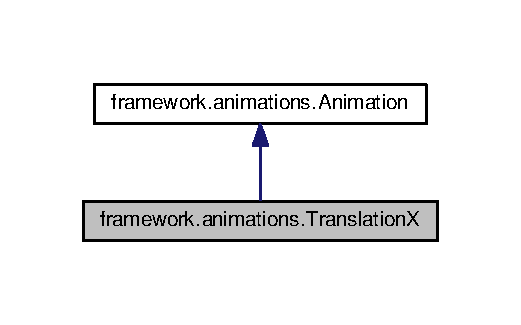
\includegraphics[width=250pt]{classframework_1_1animations_1_1TranslationX__inherit__graph}
\end{center}
\end{figure}


Collaboration diagram for framework.\+animations.\+TranslationX\+:
\nopagebreak
\begin{figure}[H]
\begin{center}
\leavevmode
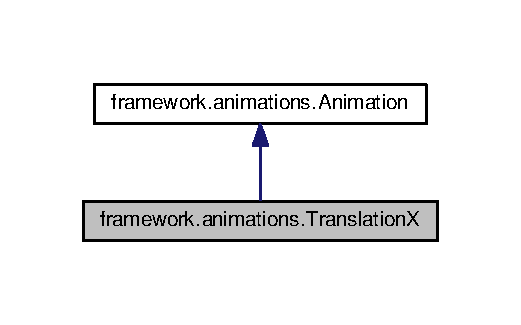
\includegraphics[width=250pt]{classframework_1_1animations_1_1TranslationX__coll__graph}
\end{center}
\end{figure}
\subsection*{Public Member Functions}
\begin{DoxyCompactItemize}
\item 
def {\bfseries \+\_\+\+\_\+init\+\_\+\+\_\+} (self, bdr\+\_\+handler, blender\+\_\+object, frames)\hypertarget{classframework_1_1animations_1_1TranslationX_a12b85b0228bb4659d43e210ba9acf226}{}\label{classframework_1_1animations_1_1TranslationX_a12b85b0228bb4659d43e210ba9acf226}

\end{DoxyCompactItemize}
\subsection*{Static Public Member Functions}
\begin{DoxyCompactItemize}
\item 
def {\bfseries get\+\_\+start\+\_\+rotation} ()\hypertarget{classframework_1_1animations_1_1TranslationX_aa9159131dbddd3a1b1c93173788f727f}{}\label{classframework_1_1animations_1_1TranslationX_aa9159131dbddd3a1b1c93173788f727f}

\item 
def {\bfseries get\+\_\+start\+\_\+position} ()\hypertarget{classframework_1_1animations_1_1TranslationX_a9468716f2fbd3688ebc3fe7ede953fee}{}\label{classframework_1_1animations_1_1TranslationX_a9468716f2fbd3688ebc3fe7ede953fee}

\end{DoxyCompactItemize}
\subsection*{Static Public Attributes}
\begin{DoxyCompactItemize}
\item 
string {\bfseries interpolation} = \textquotesingle{}L\+I\+N\+E\+AR\textquotesingle{}\hypertarget{classframework_1_1animations_1_1TranslationX_a26bcd03c9bf3c07e9f2423bc578d75d2}{}\label{classframework_1_1animations_1_1TranslationX_a26bcd03c9bf3c07e9f2423bc578d75d2}

\end{DoxyCompactItemize}


The documentation for this class was generated from the following file\+:\begin{DoxyCompactItemize}
\item 
/home/sebastian/catkin\+\_\+ws/src/animation\+\_\+render/scripts/framework/animations.\+py\end{DoxyCompactItemize}

\hypertarget{classframework_1_1animations_1_1TranslationX2}{}\section{framework.\+animations.\+Translation\+X2 Class Reference}
\label{classframework_1_1animations_1_1TranslationX2}\index{framework.\+animations.\+Translation\+X2@{framework.\+animations.\+Translation\+X2}}


Inheritance diagram for framework.\+animations.\+Translation\+X2\+:
\nopagebreak
\begin{figure}[H]
\begin{center}
\leavevmode
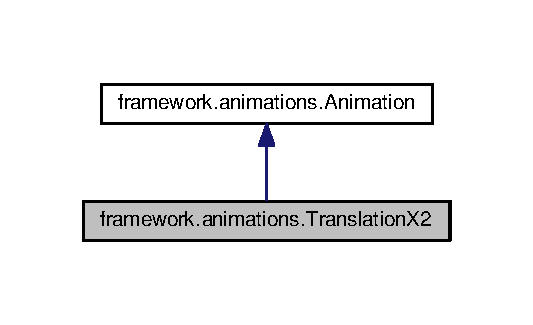
\includegraphics[width=256pt]{classframework_1_1animations_1_1TranslationX2__inherit__graph}
\end{center}
\end{figure}


Collaboration diagram for framework.\+animations.\+Translation\+X2\+:
\nopagebreak
\begin{figure}[H]
\begin{center}
\leavevmode
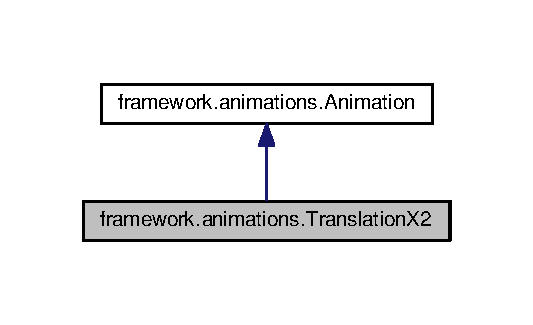
\includegraphics[width=256pt]{classframework_1_1animations_1_1TranslationX2__coll__graph}
\end{center}
\end{figure}
\subsection*{Public Member Functions}
\begin{DoxyCompactItemize}
\item 
def {\bfseries \+\_\+\+\_\+init\+\_\+\+\_\+} (self, bdr\+\_\+handler, blender\+\_\+object, frames)\hypertarget{classframework_1_1animations_1_1TranslationX2_a7282fa4205c40d00a787ae5ae2454ebb}{}\label{classframework_1_1animations_1_1TranslationX2_a7282fa4205c40d00a787ae5ae2454ebb}

\end{DoxyCompactItemize}
\subsection*{Static Public Member Functions}
\begin{DoxyCompactItemize}
\item 
def {\bfseries get\+\_\+start\+\_\+rotation} ()\hypertarget{classframework_1_1animations_1_1TranslationX2_a30a5afe964abe1c5eb5014439f444a0d}{}\label{classframework_1_1animations_1_1TranslationX2_a30a5afe964abe1c5eb5014439f444a0d}

\item 
def {\bfseries get\+\_\+start\+\_\+position} ()\hypertarget{classframework_1_1animations_1_1TranslationX2_afb4169d1362618f8668fd70faf2999e0}{}\label{classframework_1_1animations_1_1TranslationX2_afb4169d1362618f8668fd70faf2999e0}

\end{DoxyCompactItemize}
\subsection*{Static Public Attributes}
\begin{DoxyCompactItemize}
\item 
string {\bfseries interpolation} = \textquotesingle{}Q\+U\+AD\textquotesingle{}\hypertarget{classframework_1_1animations_1_1TranslationX2_a37ef9998ae63a4c452b82aa7ada36889}{}\label{classframework_1_1animations_1_1TranslationX2_a37ef9998ae63a4c452b82aa7ada36889}

\end{DoxyCompactItemize}


The documentation for this class was generated from the following file\+:\begin{DoxyCompactItemize}
\item 
/home/sebastian/catkin\+\_\+ws/src/animation\+\_\+render/scripts/framework/animations.\+py\end{DoxyCompactItemize}

\hypertarget{classframework_1_1animations_1_1TranslationXY}{}\section{framework.\+animations.\+Translation\+XY Class Reference}
\label{classframework_1_1animations_1_1TranslationXY}\index{framework.\+animations.\+Translation\+XY@{framework.\+animations.\+Translation\+XY}}


Inheritance diagram for framework.\+animations.\+Translation\+XY\+:
\nopagebreak
\begin{figure}[H]
\begin{center}
\leavevmode
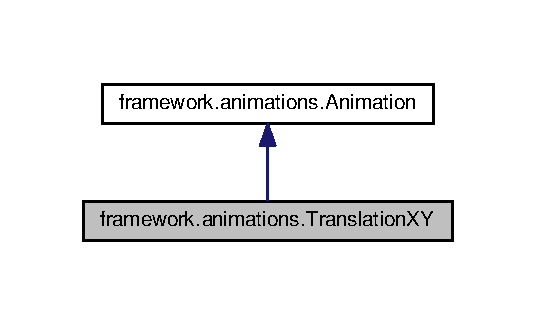
\includegraphics[width=257pt]{classframework_1_1animations_1_1TranslationXY__inherit__graph}
\end{center}
\end{figure}


Collaboration diagram for framework.\+animations.\+Translation\+XY\+:
\nopagebreak
\begin{figure}[H]
\begin{center}
\leavevmode
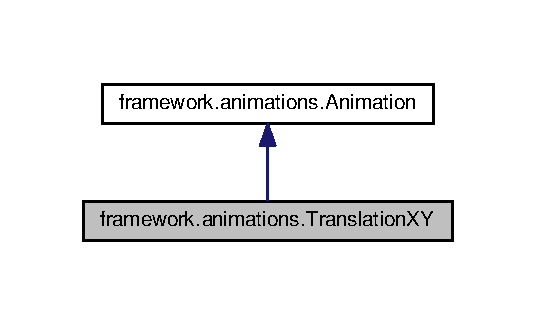
\includegraphics[width=257pt]{classframework_1_1animations_1_1TranslationXY__coll__graph}
\end{center}
\end{figure}
\subsection*{Public Member Functions}
\begin{DoxyCompactItemize}
\item 
def {\bfseries \+\_\+\+\_\+init\+\_\+\+\_\+} (self, bdr\+\_\+handler, blender\+\_\+object, frames)\hypertarget{classframework_1_1animations_1_1TranslationXY_aed3853e74e9461d11acaabf6d9112b58}{}\label{classframework_1_1animations_1_1TranslationXY_aed3853e74e9461d11acaabf6d9112b58}

\end{DoxyCompactItemize}
\subsection*{Static Public Member Functions}
\begin{DoxyCompactItemize}
\item 
def {\bfseries get\+\_\+start\+\_\+rotation} ()\hypertarget{classframework_1_1animations_1_1TranslationXY_abe4e71aa431884d0761616f2da27c652}{}\label{classframework_1_1animations_1_1TranslationXY_abe4e71aa431884d0761616f2da27c652}

\item 
def {\bfseries get\+\_\+start\+\_\+position} ()\hypertarget{classframework_1_1animations_1_1TranslationXY_a7af50f92d7c771c106209d8a5508fafa}{}\label{classframework_1_1animations_1_1TranslationXY_a7af50f92d7c771c106209d8a5508fafa}

\end{DoxyCompactItemize}
\subsection*{Static Public Attributes}
\begin{DoxyCompactItemize}
\item 
string {\bfseries interpolation} = \textquotesingle{}L\+I\+N\+E\+AR\textquotesingle{}\hypertarget{classframework_1_1animations_1_1TranslationXY_a91d5fcf6ca9e859055cd1d107b16cf36}{}\label{classframework_1_1animations_1_1TranslationXY_a91d5fcf6ca9e859055cd1d107b16cf36}

\end{DoxyCompactItemize}


The documentation for this class was generated from the following file\+:\begin{DoxyCompactItemize}
\item 
/home/sebastian/catkin\+\_\+ws/src/animation\+\_\+render/scripts/framework/animations.\+py\end{DoxyCompactItemize}

\hypertarget{classframework_1_1animations_1_1TranslationXYrotated}{}\section{framework.\+animations.\+Translation\+X\+Yrotated Class Reference}
\label{classframework_1_1animations_1_1TranslationXYrotated}\index{framework.\+animations.\+Translation\+X\+Yrotated@{framework.\+animations.\+Translation\+X\+Yrotated}}


Inheritance diagram for framework.\+animations.\+Translation\+X\+Yrotated\+:
\nopagebreak
\begin{figure}[H]
\begin{center}
\leavevmode
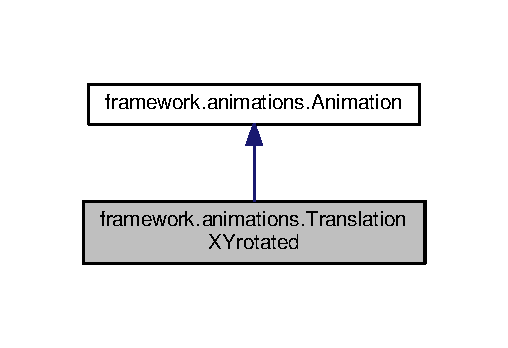
\includegraphics[width=244pt]{classframework_1_1animations_1_1TranslationXYrotated__inherit__graph}
\end{center}
\end{figure}


Collaboration diagram for framework.\+animations.\+Translation\+X\+Yrotated\+:
\nopagebreak
\begin{figure}[H]
\begin{center}
\leavevmode
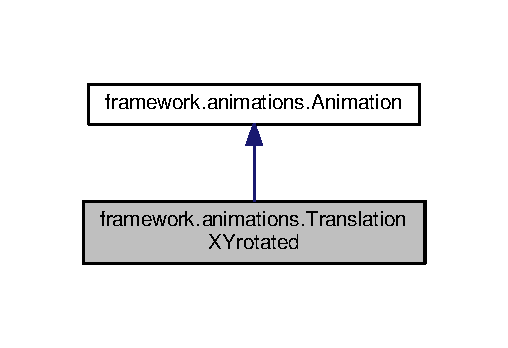
\includegraphics[width=244pt]{classframework_1_1animations_1_1TranslationXYrotated__coll__graph}
\end{center}
\end{figure}
\subsection*{Public Member Functions}
\begin{DoxyCompactItemize}
\item 
def {\bfseries \+\_\+\+\_\+init\+\_\+\+\_\+} (self, bdr\+\_\+handler, blender\+\_\+object, frames)\hypertarget{classframework_1_1animations_1_1TranslationXYrotated_aa74ae01288abcc53255b3e98b9cb935a}{}\label{classframework_1_1animations_1_1TranslationXYrotated_aa74ae01288abcc53255b3e98b9cb935a}

\end{DoxyCompactItemize}
\subsection*{Static Public Member Functions}
\begin{DoxyCompactItemize}
\item 
def {\bfseries get\+\_\+start\+\_\+position} ()\hypertarget{classframework_1_1animations_1_1TranslationXYrotated_adc844f54e26e44175be58d5d96ab5c97}{}\label{classframework_1_1animations_1_1TranslationXYrotated_adc844f54e26e44175be58d5d96ab5c97}

\item 
def {\bfseries get\+\_\+start\+\_\+rotation} ()\hypertarget{classframework_1_1animations_1_1TranslationXYrotated_ac9956bceaaa525d55482d8c8114c494b}{}\label{classframework_1_1animations_1_1TranslationXYrotated_ac9956bceaaa525d55482d8c8114c494b}

\end{DoxyCompactItemize}
\subsection*{Static Public Attributes}
\begin{DoxyCompactItemize}
\item 
string {\bfseries interpolation} = \textquotesingle{}Q\+U\+AD\textquotesingle{}\hypertarget{classframework_1_1animations_1_1TranslationXYrotated_a917101a647c65a3f4becab7f4470c018}{}\label{classframework_1_1animations_1_1TranslationXYrotated_a917101a647c65a3f4becab7f4470c018}

\end{DoxyCompactItemize}


The documentation for this class was generated from the following file\+:\begin{DoxyCompactItemize}
\item 
/home/sebastian/catkin\+\_\+ws/src/animation\+\_\+render/scripts/framework/animations.\+py\end{DoxyCompactItemize}

\hypertarget{classframework_1_1animations_1_1TranslationY}{}\section{framework.\+animations.\+TranslationY Class Reference}
\label{classframework_1_1animations_1_1TranslationY}\index{framework.\+animations.\+TranslationY@{framework.\+animations.\+TranslationY}}


Inheritance diagram for framework.\+animations.\+TranslationY\+:
\nopagebreak
\begin{figure}[H]
\begin{center}
\leavevmode
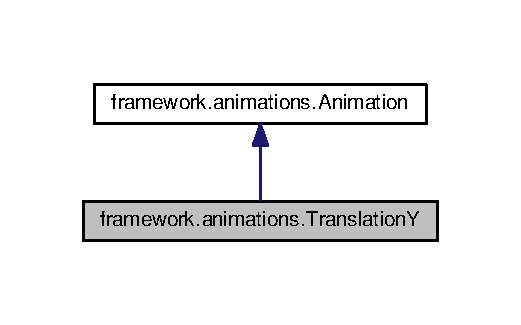
\includegraphics[width=250pt]{classframework_1_1animations_1_1TranslationY__inherit__graph}
\end{center}
\end{figure}


Collaboration diagram for framework.\+animations.\+TranslationY\+:
\nopagebreak
\begin{figure}[H]
\begin{center}
\leavevmode
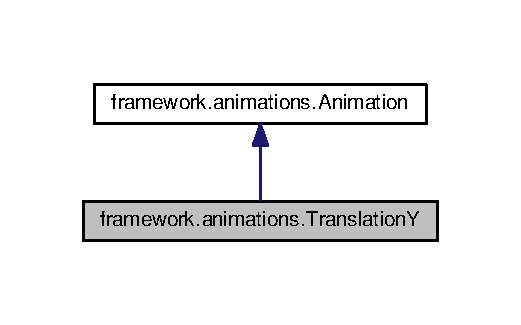
\includegraphics[width=250pt]{classframework_1_1animations_1_1TranslationY__coll__graph}
\end{center}
\end{figure}
\subsection*{Public Member Functions}
\begin{DoxyCompactItemize}
\item 
def {\bfseries \+\_\+\+\_\+init\+\_\+\+\_\+} (self, bdr\+\_\+handler, blender\+\_\+object, frames)\hypertarget{classframework_1_1animations_1_1TranslationY_a17b43b4fcbff26dff84370849d650287}{}\label{classframework_1_1animations_1_1TranslationY_a17b43b4fcbff26dff84370849d650287}

\end{DoxyCompactItemize}
\subsection*{Static Public Member Functions}
\begin{DoxyCompactItemize}
\item 
def {\bfseries get\+\_\+start\+\_\+rotation} ()\hypertarget{classframework_1_1animations_1_1TranslationY_a44ebc6fbcb081c5701f26573bb363af1}{}\label{classframework_1_1animations_1_1TranslationY_a44ebc6fbcb081c5701f26573bb363af1}

\item 
def {\bfseries get\+\_\+start\+\_\+position} ()\hypertarget{classframework_1_1animations_1_1TranslationY_a15c74f762cda5d8a2cb79525fd5e079a}{}\label{classframework_1_1animations_1_1TranslationY_a15c74f762cda5d8a2cb79525fd5e079a}

\end{DoxyCompactItemize}
\subsection*{Static Public Attributes}
\begin{DoxyCompactItemize}
\item 
string {\bfseries interpolation} = \textquotesingle{}Q\+U\+AD\textquotesingle{}\hypertarget{classframework_1_1animations_1_1TranslationY_af9a508ceb9210bba0e29bf469217bf70}{}\label{classframework_1_1animations_1_1TranslationY_af9a508ceb9210bba0e29bf469217bf70}

\end{DoxyCompactItemize}


The documentation for this class was generated from the following file\+:\begin{DoxyCompactItemize}
\item 
/home/sebastian/catkin\+\_\+ws/src/animation\+\_\+render/scripts/framework/animations.\+py\end{DoxyCompactItemize}

\hypertarget{classframework_1_1animations_1_1TranslationZ}{}\section{framework.\+animations.\+TranslationZ Class Reference}
\label{classframework_1_1animations_1_1TranslationZ}\index{framework.\+animations.\+TranslationZ@{framework.\+animations.\+TranslationZ}}


Inheritance diagram for framework.\+animations.\+TranslationZ\+:
\nopagebreak
\begin{figure}[H]
\begin{center}
\leavevmode
\includegraphics[width=250pt]{classframework_1_1animations_1_1TranslationZ__inherit__graph}
\end{center}
\end{figure}


Collaboration diagram for framework.\+animations.\+TranslationZ\+:
\nopagebreak
\begin{figure}[H]
\begin{center}
\leavevmode
\includegraphics[width=250pt]{classframework_1_1animations_1_1TranslationZ__coll__graph}
\end{center}
\end{figure}
\subsection*{Public Member Functions}
\begin{DoxyCompactItemize}
\item 
def {\bfseries \+\_\+\+\_\+init\+\_\+\+\_\+} (self, bdr\+\_\+handler, blender\+\_\+object, frames)\hypertarget{classframework_1_1animations_1_1TranslationZ_a2cb51ff4f2413ec338b206237ea008b8}{}\label{classframework_1_1animations_1_1TranslationZ_a2cb51ff4f2413ec338b206237ea008b8}

\end{DoxyCompactItemize}
\subsection*{Static Public Member Functions}
\begin{DoxyCompactItemize}
\item 
def {\bfseries get\+\_\+start\+\_\+position} ()\hypertarget{classframework_1_1animations_1_1TranslationZ_a20f747900e64a283bb3531b4c9dbc6c7}{}\label{classframework_1_1animations_1_1TranslationZ_a20f747900e64a283bb3531b4c9dbc6c7}

\item 
def {\bfseries get\+\_\+start\+\_\+rotation} ()\hypertarget{classframework_1_1animations_1_1TranslationZ_a25302431d774870bdcff75ef7fd3bd78}{}\label{classframework_1_1animations_1_1TranslationZ_a25302431d774870bdcff75ef7fd3bd78}

\end{DoxyCompactItemize}
\subsection*{Static Public Attributes}
\begin{DoxyCompactItemize}
\item 
string {\bfseries interpolation} = \textquotesingle{}L\+I\+N\+E\+AR\textquotesingle{}\hypertarget{classframework_1_1animations_1_1TranslationZ_ab4af6e78253c99e8926aa5066112a79c}{}\label{classframework_1_1animations_1_1TranslationZ_ab4af6e78253c99e8926aa5066112a79c}

\end{DoxyCompactItemize}


The documentation for this class was generated from the following file\+:\begin{DoxyCompactItemize}
\item 
/home/sebastian/catkin\+\_\+ws/src/animation\+\_\+render/scripts/framework/animations.\+py\end{DoxyCompactItemize}

\hypertarget{structVideoOptions}{}\section{Video\+Options Struct Reference}
\label{structVideoOptions}\index{Video\+Options@{Video\+Options}}
\subsection*{Public Attributes}
\begin{DoxyCompactItemize}
\item 
int {\bfseries width}\hypertarget{structVideoOptions_ad47a8f090805a349fc6f200d21c71549}{}\label{structVideoOptions_ad47a8f090805a349fc6f200d21c71549}

\item 
int {\bfseries height}\hypertarget{structVideoOptions_a9031cd944b0dd5c6e6c135afb0db5b26}{}\label{structVideoOptions_a9031cd944b0dd5c6e6c135afb0db5b26}

\item 
int {\bfseries fps}\hypertarget{structVideoOptions_a73674e8c88aa4f459c127511be49c0b2}{}\label{structVideoOptions_a73674e8c88aa4f459c127511be49c0b2}

\item 
int {\bfseries frames}\hypertarget{structVideoOptions_a644e265827a217ce4e7eabc2f226904d}{}\label{structVideoOptions_a644e265827a217ce4e7eabc2f226904d}

\item 
double {\bfseries sensor\+\_\+width}\hypertarget{structVideoOptions_ae16bb057999c1278e501d27f35cc0b85}{}\label{structVideoOptions_ae16bb057999c1278e501d27f35cc0b85}

\item 
double {\bfseries focal\+\_\+length}\hypertarget{structVideoOptions_a13b51ddc57b1ab2a3696d9edbcb74107}{}\label{structVideoOptions_a13b51ddc57b1ab2a3696d9edbcb74107}

\end{DoxyCompactItemize}


The documentation for this struct was generated from the following file\+:\begin{DoxyCompactItemize}
\item 
/home/sebastian/catkin\+\_\+ws/src/animation\+\_\+render/src/pythoncaller.\+h\end{DoxyCompactItemize}

\hypertarget{classVideoStream}{}\section{Video\+Stream Class Reference}
\label{classVideoStream}\index{Video\+Stream@{Video\+Stream}}
\subsection*{Public Member Functions}
\begin{DoxyCompactItemize}
\item 
{\bfseries Video\+Stream} (ros\+::\+Node\+Handle rosH)\hypertarget{classVideoStream_ab3287a533657a03cfb293793962faf3c}{}\label{classVideoStream_ab3287a533657a03cfb293793962faf3c}

\item 
bool \hyperlink{classVideoStream_ab8d19b1d9d1156fb9d12ada5ce6409bb}{open\+Stream} (std\+::string path, \hyperlink{structVideoOptions}{Video\+Options} options)
\begin{DoxyCompactList}\small\item\em open\+Stream Reads video file and streams it over camera topic \end{DoxyCompactList}\end{DoxyCompactItemize}


\subsection{Member Function Documentation}
\index{Video\+Stream@{Video\+Stream}!open\+Stream@{open\+Stream}}
\index{open\+Stream@{open\+Stream}!Video\+Stream@{Video\+Stream}}
\subsubsection[{\texorpdfstring{open\+Stream(std\+::string path, Video\+Options options)}{openStream(std::string path, VideoOptions options)}}]{\setlength{\rightskip}{0pt plus 5cm}bool Video\+Stream\+::open\+Stream (
\begin{DoxyParamCaption}
\item[{std\+::string}]{path, }
\item[{{\bf Video\+Options}}]{options}
\end{DoxyParamCaption}
)}\hypertarget{classVideoStream_ab8d19b1d9d1156fb9d12ada5ce6409bb}{}\label{classVideoStream_ab8d19b1d9d1156fb9d12ada5ce6409bb}


open\+Stream Reads video file and streams it over camera topic 


\begin{DoxyParams}{Parameters}
{\em path} & Path of video file \\
\hline
\end{DoxyParams}


The documentation for this class was generated from the following files\+:\begin{DoxyCompactItemize}
\item 
/home/sebastian/catkin\+\_\+ws/src/animation\+\_\+render/src/videostream.\+h\item 
/home/sebastian/catkin\+\_\+ws/src/animation\+\_\+render/src/videostream.\+cpp\end{DoxyCompactItemize}

%--- End generated contents ---

% Index
\backmatter
\newpage
\phantomsection
\clearemptydoublepage
\addcontentsline{toc}{chapter}{Index}
\printindex

\end{document}
